\RequirePackage[l2tabu, orthodox]{nag}


% ------ Main document class specification ------
% The draft option here prevents images being inserted,
%  and adds chunky black bars to boxes that are exceeding 
%  the page width (to show that they are).
% The oneside option can optionally be replaced by twoside if
%  you intend to print double-sided. Note that this is
%  *specifically permitted* by the UCL thesis formatting
%  guidelines.
%
% Valid options in terms of type are:
%  phd
%  mres
%  mphil
%\documentclass[12pt,phd,draft,a4paper,oneside]{ucl_thesis}
\documentclass[12pt,phd,a4paper,oneside]{ucl_thesis}


% Package configuration:
%  LaTeX uses "packages" to add extra commands and features.
%  There are quite a few useful ones, so we've put them in a 
%   separate file.
% -------- Packages --------

% This package just gives you a quick way to dump in some sample text.
% You can remove it -- it's just here for the examples.
\usepackage{blindtext}
\usepackage[english]{babel} 
% This package means empty pages (pages with no text) won't get stuff
%  like chapter names at the top of the page. It's mostly cosmetic.
\usepackage{emptypage}

% The graphicx package adds the \includegraphics command,
%  which is your basic command for adding a picture.
\usepackage{graphicx}

% This command is provided by the graphicx package, and 
%  controls the default dpi resolution of images you use.
%  72 is the default, but 300 is more normal, and 600 is
%  as good as you can expect to be able to get on normal paper.
\pdfimageresolution=300


% The float package improves LaTeX's handling of floats,
%  and also adds the option to *force* LaTeX to put the float
%  HERE, with the [H] option to the float environment.
\usepackage{float}

% The amsmath package enhances the various ways of including
%  maths, including adding the align environment for aligned
%  equations.
\usepackage{amsmath}

% Use these two packages together -- they define symbols
%  for e.g. units that you can use in both text and math mode.
\usepackage{gensymb}
\usepackage{textcomp}
% You may also want the units package for making little
%  fractions for unit specifications.
%\usepackage{units}


% The setspace package lets you use 1.5-sized or double line spacing.
\usepackage{setspace}
\setstretch{1.5}

% That just does body text -- if you want to expand *everything*,
%  including footnotes and tables, use this instead:
%\renewcommand{\baselinestretch}{1.5}


% PGFPlots is either a really clunky or really good way to add graphs
%  into your document, depending on your point of view.
% There's waaaaay too much information on using this to cover here,
%  so, you might want to start here:
%   http://pgfplots.sourceforge.net/
%  or here:
%   http://pgfplots.sourceforge.net/pgfplots.pdf
%\usepackage{pgfplots}
%\pgfplotsset{compat=1.3} % <- this fixed axis labels in the version I was using

% PGFPlotsTable can help you make tables a little more easily than
%  usual in LaTeX.
% If you're going to have to paste data in a lot, I'd suggest using it.
%  You might want to start with the manual, here:
%  http://pgfplots.sourceforge.net/pgfplotstable.pdf
%\usepackage{pgfplotstable}

% These settings are also recommended for using with pgfplotstable.
%\pgfplotstableset{
%	% these columns/<colname>/.style={<options>} things define a style
%	% which applies to <colname> only.
%	empty cells with={--}, % replace empty cells with '--'
%	every head row/.style={before row=\toprule,after row=\midrule},
%	every last row/.style={after row=\bottomrule}
%}


% The mhchem package provides chemistry formula typesetting commands
%  e.g. \ce{H2O}
%\usepackage[version=3]{mhchem}

% And the chemfig package gives a weird command for adding Lewis 
%  diagrams, for e.g. organic molecules
%\usepackage{chemfig}

% The linenumbers command from the lineno package adds line numbers
%  alongside your text that can be useful for discussing edits 
%  in drafts.
% Remove or comment out the command for proper versions.
%\usepackage[modulo]{lineno}
% \linenumbers 


% Alternatively, you can use the ifdraft package to let you add
%  commands that will only be used in draft versions
%\usepackage{ifdraft}

% For example, the following adds a watermark if the draft mode is on.
%\ifdraft{
%  \usepackage{draftwatermark}
%  \SetWatermarkText{\shortstack{\textsc{Draft Mode}\\ \strut \\ \strut \\ \strut}}
%  \SetWatermarkScale{0.5}
%  \SetWatermarkAngle{90}
%}


% The multirow package adds the option to make cells span 
%  rows in tables.
\usepackage{multirow}


% Subfig allows you to create figures within figures, to, for example,
%  make a single figure with 4 individually labeled and referenceable
%  sub-figures.
% It's quite fiddly to use, so check the documentation.
%\usepackage{subfig}

% The natbib package allows book-type citations commonly used in
%  longer works, and less commonly in science articles (IME).
% e.g. (Saucer et al., 1993) rather than [1]
% More details are here: http://merkel.zoneo.net/Latex/natbib.php
%\usepackage{natbib}

% The bibentry package (along with the \nobibliography* command)
%  allows putting full reference lines inline.
%  See: 
%   http://tex.stackexchange.com/questions/2905/how-can-i-list-references-from-bibtex-file-in-line-with-commentary
\usepackage{bibentry} 

% The isorot package allows you to put things sideways 
%  (or indeed, at any angle) on a page.
% This can be useful for wide graphs or other figures.
%\usepackage{isorot}

% The caption package adds more options for caption formatting.
% This set-up makes hanging labels, makes the caption text smaller
%  than the body text, and makes the label bold.
% Highly recommended.
\usepackage[format=hang,font=small,labelfont=bf]{caption}

% If you're getting into defining your own commands, you might want
%  to check out the etoolbox package -- it defines a few commands
%  that can make it easier to make commands robust.
\usepackage{etoolbox}
\usepackage[english]{babel}
\usepackage[utf8]{inputenc}

%Includes "References" in the table of contents
\usepackage[nottoc]{tocbibind}
\usepackage[utf8]{inputenc}
\usepackage[english]{babel}
\usepackage{graphicx}
\graphicspath{{images/}}
\DeclareGraphicsExtensions{.png,.pdf}
\usepackage{subcaption}


% Sets up links within your document, for e.g. contents page entries
%  and references, and also PDF metadata.
% You should edit this!
%%
%% This file uses the hyperref package to make your thesis have metadata embedded in the PDF, 
%%  and also adds links to be able to click on references and contents page entries to go to 
%%  the pages.
%%

% Some hacks are necessary to make bibentry and hyperref play nicely.
% See: http://tex.stackexchange.com/questions/65348/clash-between-bibentry-and-hyperref-with-bibstyle-elsart-harv
\usepackage{bibentry}
\makeatletter\let\saved@bibitem\@bibitem\makeatother
\usepackage[pdftex,hidelinks]{hyperref}
\makeatletter\let\@bibitem\saved@bibitem\makeatother
\makeatletter
\AtBeginDocument{
    \hypersetup{
        pdfsubject={Thesis Subject},
        pdfkeywords={Thesis Keywords},
        pdfauthor={Author},
        pdftitle={Title},
    }
}
\makeatother
    


% And then some settings in separate files.
% These settings are from:
%  http://mintaka.sdsu.edu/GF/bibliog/latex/floats.html

% They give LaTeX more options on where to put your figures, and may
%  mean that fewer of your figures end up at the tops of pages far
%  away from the thing they're related to.

% Alters some LaTeX defaults for better treatment of figures:
% See p.105 of "TeX Unbound" for suggested values.
% See pp. 199-200 of Lamport's "LaTeX" book for details.

%   General parameters, for ALL pages:
\renewcommand{\topfraction}{0.9}	% max fraction of floats at top
\renewcommand{\bottomfraction}{0.8}	% max fraction of floats at bottom

%   Parameters for TEXT pages (not float pages):
\setcounter{topnumber}{2}
\setcounter{bottomnumber}{2}
\setcounter{totalnumber}{4}     % 2 may work better
\setcounter{dbltopnumber}{2}    % for 2-column pages
\renewcommand{\dbltopfraction}{0.9}	% fit big float above 2-col. text
\renewcommand{\textfraction}{0.07}	% allow minimal text w. figs

%   Parameters for FLOAT pages (not text pages):
\renewcommand{\floatpagefraction}{0.7}	% require fuller float pages
% N.B.: floatpagefraction MUST be less than topfraction !!
\renewcommand{\dblfloatpagefraction}{0.7}	% require fuller float pages

% remember to use [htp] or [htpb] for placement,
% e.g. 
%  \begin{figure}[htp]
%   ...
%  \end{figure} % For things like figures and tables
\bibliographystyle{unsrt}   % For bibliographies

% Title Settings
\setcounter{secnumdepth}{3}
\setcounter{tocdepth}{3}
\title{Counting Features for Cross Domain Learning}
\author{Xinyang Gao}
\department{Department of Computer Science}


\begin{document}



\nobibliography*
% This is a dumb trick that works with the bibentry package to let
%  you put bibliography entries whereever you like.
% I used this to put references to papers a chapter's work was 
%  published in at the end of that chapter.
% For more information, see: http://stefaanlippens.net/bibentry

% If you haven't finished making your full BibTex file yet, you
%  might find this useful -- it'll just replace all your
%  citations with little superscript notes.
% Uncomment to use.
%\renewcommand{\cite}[1]{\emph{\textsuperscript{[#1]}}}

% At last, content! Remember filenames are case-sensitive and 
%  *must not* include spaces.
\maketitle
\makedeclaration

\begin{abstract} % 300 word limit
In Click-Through Rate (CTR) estimation problems for online advertising, besides the pursue of fancy models and algorithms, feature engineering is informal but absolutely vital to its success. Traditionally, in industry, the generation, combination and transformation of effective one-hot encoded features are always conducted manually, which is time-consuming and labor-intensive. Even worse, in the age of big data, astronomical user impressions lead to enormous unique binary features, the industry is having an urgent demand for the type of ad feature which are light-weight, scalable and auto-generated. In this paper, we propose the concept of \textit{counting features} which constitutes the \textit{Frequency} and \textit{Average CTR} information of all the items in each field, representing the statistical characteristics of the dataset. Further, we exploit the performance of counting feature using valuable real world data provided by Adform. AUC and RMSE are used to evaluate its performance in CTR prediction showing that the its CTR prediction accuracy when utilising non-linear model is comparable to that of binary feature utilising linear model. Finally, we apply counting feature on \textit{cross-domain learning} problem, with the goal to solve the canonical \textit{cold start} problem for online adverting CTR prediction, so that knowledge from old ad campaigns can be directly used by new campaign with minimal updates for the classifiers. We show that the distributions of the conditional probability \(Pr(Click|Feature)\) are alike among different campaigns, the variability of classifiers can be decreased when using counting feature against binary feature, thus increasing the generality of CTR prediction model and making \textit{direct cross domain CTR prediction model} possible. Experiment results show counting feature's performance is superior to binary feature in cold start problem. 
\end{abstract}

\begin{acknowledgements}
I would like to pay my best respect to my supervisor Dr. Jun Wang who provides invaluable guidance and support to my research, only with the ongoing creative and solid suggestions from Dr. Jun can I finalize my Msc project.

I also want to tribute to the PHD candidate, Weinan Zhang, who provides precious help for my mathematical deduction work and experiment implementation, as the final year PHD who is up to his neck, Weinan still takes a lot of time off in supporting me, I highly appreciate his guidance.

The senior fellow student Xuyang Wu also provides me with many helps in setting up the system of \textit{OpenBidder}\footnote{http://www.openbidder.com/}, I learned a lot of engineering work for RTB system from him, I would like to thank him.

Last but not least, I would absolutely thank 	
Mr.Thomas Furmston and Mr.Edward Snelson from Adform company who not only provide me with valuable real world advertising data, but also enormous guidance for my project, I will show my best respects to them.
\end{acknowledgements}

\setcounter{tocdepth}{2} 
% Setting this higher means you get contents entries for
%  more minor section headers.

\tableofcontents
\listoffigures
\listoftables


\chapter{Introduction}
\label{chapterlabel1}

Real Time Bidding (RTB)\footnote{https://en.wikipedia.org/wiki/Real-time_bidding} has recently become paradigm for online advertising which subversively transformed the whole ecosystem. Unlike traditional contextual advertising, RTB allows advertisers to bid for each of the impression based on user profile data, but not only the contextual web data. Demand side platform (DSP)\footnote{https://en.wikipedia.org/wiki/Demand-side_platform}'s responsibility is to help advertisers optimize their bidding strategy in order to maximize the return of investment (ROI) for its clients. When a potential advertisement audience visits a webpage, a bid request will be sent to DSP who will decide a price to bid for the webspace slot. Economically we know that \(Profit = Revenue - Cost\), in which cost is the winning price for the advertiser, called \textit{Cost-Per-Click} (CPC), revenue, or \textit{Earning per Click} (EPC) is the expected return that can be obtained from the potential advertisement audience based on auction winning function which can be found in \cite{zhang2014optimal}. Briefly speaking, the revenue can be yielded by the product of the expected click per impression and EPC. The pursuit of maximum profit can be achieved by either increasing revenue or decreasing the cost, accurate CTR prediction is crucial to this goal which determines the expected potential revenue for the impression and according bidding price. 

CTR prediction has been researched extensively in recent years academically and industrially, it is especially important to the industry since the CTR prediction impacts the user experience and advertisers' revenue. Microsoft \cite{graepel2010web} has proposed a novel way for CTR prediction model on Sponsored Search in Microsoft’s Bing search engine, Gaussian beliefs across the weights of the model can be maintained and the weights are updated online based on approximate message passing. Facebook \cite{he2014practical} also demonstrates their success on online advertisement CTR prediction. With the combination of decision trees and logistic regression, and other techniques such as feature selection, learning rate schema, data freshness, and data sampling, the performance of CTR prediction can be largely increased.  

However, most current work are restricted to the scope of enhancement of model formation, parameter adjustment and algorithm optimization, but according to Facebook recent report \cite{facebook2015}, the \textit{experimental paradigm is reaching its limits}, in Machine Learning (ML) the experimental paradigm means the procedure of  (i) Setting aside test dataset, (ii) Estimating prediction function using training dataset, and (iii) Measure final performance using testing dataset. In the last a few decades this single paradigm dominates the research in the field of machine learning, which is on the premise that the data used are gathered correctly without bias. In such case, data plays more significant role in enhancing performance of ML application than feature and algorithm, as shown in Figure ~\ref{fig:datai}

\begin{figure}[h]
\centering
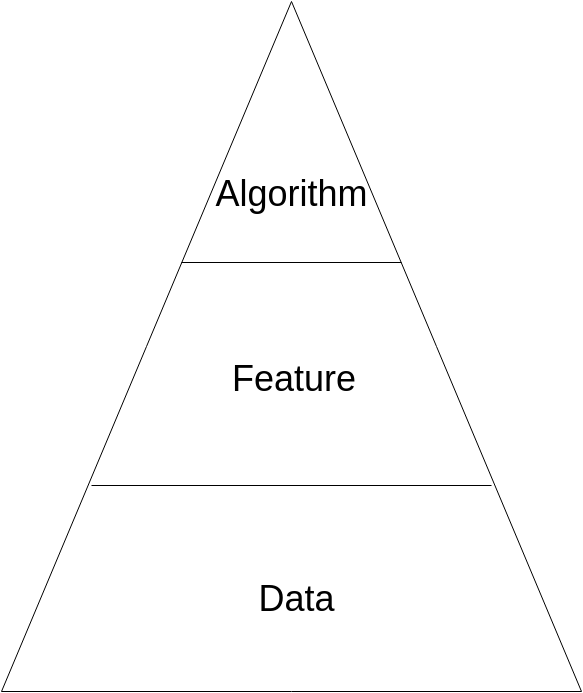
\includegraphics[scale=1.5]{data.png}
\caption{Importance of factors to the performance of ML application}
\label{fig:datai}
\end{figure}

However, in the age of big data \cite{lohr2012age}, large datasets are collected automatically so bias are inevitable among the datasets, therefore, unrealistic results will be obtained from training/testing dataset using the above \textit{experimental paradigm} \cite{torralba2011unbiased}. So for most current researches the models are trained and tested based on one single dataset, the classifiers learned can only work under a certain statistical distribution of the data. Only if with the updates of the model, can the classifiers trained from the old campaigns be applied to new campaigns in the concept of online advertisement. Therefore, under the situation that the advertising data from different advertiser campaigns behave differently and largely biased, according to the idea in \cite{threethings2015} and \cite{domingos2012few}, representation of the data will be essential for machine learning algorithms. More informative data extracted from the dataset, more improvement in performance of the algorithm can be obtained, since digging out the insights from the dataset means filtering out the redundant information which are irrelevant to the prediction task. Therefore, we will focus on the process of \textit{Feature Extraction} or \textit{Feature Engineering} to reach the goal that, 
\begin{itemize}
\item  the new feature space is low dimensional to avoid the \textit{curse of dimensionality} which will be common in the age of \textit{Big Data}
\item the new feature space is informative and the irrelevant data are got rid of, while the performance of prediction task is still comparable to that of traditional binary feature.
\item  the new feature space can help partly solve the \textit{cold start} problem to generalize the model among different campaigns.
\end{itemize}

In this paper we postulate the concept of \textit{Counting Feature} which is the first time, to satisfy the above three requirements. To shortly introduce counting feature, the counting feature of each \textit{field} in the meta ad data is composed of two parts, i.e., \textit{frequency feature} and \textit{average CTR feature}. Frequency feature represents the marginal distribution of the items in the field, and average CTR feature shows the conditional distribution of the clicks on the items in that field. For example, for the field of \textit{City} in meta data there are 500 different cities, if Beijing appears 100,000 times in the dataset with a total number of 1,000,000 impressions, which in total lead to 100 clicks from clients, Hong Kong appears 50,000 times, which also bring 100 clicks for the advertiser. Then in the concept of counting feature, there will be only two features generated from this field of \textit{city}, and the counting values are continuous such as Beijing with frequency counting value 0.1 and average CTR counting value 0.001, Hong Kong with frequency counting value 0.05 and average CTR counting value 0.002. But for binary feature which is encoded into one-hot feature, there will be 500 unique feature generated from the field \textit{city} with only one feature as 1 and others as 0 for each impression, which is sparse and redundant. The goal of low dimension feature space can be achieved by the construction of counting feature based on the statistical property of the dataset. 

What's more, admitting the existence of the bias in the dataset, we prove that the performance of counting feature using non-linear logistic regression model is comparable to that of binary feature using linear logistic regression model. Generally, binary features can be widely used in linear regression based estimators such as logistic regression. Counting features can be used in the tree models such as random forest or gradient boosting regression tree for their continuity property, and they can achieve similar performance in the two situations. To the best of our knowledge, there is no work extensively studying the comparison and relationship of these two kinds of features. Particularly,this is the first time that counting feature based CTR estimation is discussed.  

The classical \textit{Cold Start} problem for online learning is the biggest barrier to meet the 3rd requirement. In the scope of online advertising CTR prediction, cold start problem can be interprated that with the knowledge from old advertisement campaigns, how to apply them to new campaigns which are lack of information initially, in order to avoid repetitive work of data collection and model construction, to make sure that large-scale industry online implementation of CTR prediction system feasible. Most of the current research such as \cite{mohan2011web} \cite{chu2011unbiased} \cite{he2014practical} and \cite{mcmahan2013ad} regard it as an active learning problem, the parameters of the model are regarded as a probability distribution and with the help of Bayesian probit method, the parameters can be updated as new data comes in thus enhancing the precision of CTR prediction for new campaign. However, in the time of big data, online data stream is extremely huge which cost resources and time for the updating of the model. In our work, we try to build a general cross domain model which can be used for each advertisement campaign without the tedious process of model updating. Different from binary feature based model, in which the number of features is variable and feature value is fixed (0 and 1), counting feature benefits from the truth that its number of features is static and feature value can be variable, thus transforming the variability form weight space of the model to the feature space. The counting feature value for each item in each field can be updated with the increasing amount of statistical information gathered from the new campaign. We prove that counting feature performs significantly better than binary feature with high dimensions in terms of cross-domain CTR prediction, the experimental results also show that with the increasing volume of statistical information gathered from new campaign, AUC increases accordingly for counting feature model but with no impact on binary feature based model.

In summary, the contributions of this paper are as follows:
\begin{itemize}
\item We find the relation between binary feature and counting feature and show that their performances for CTR prediction are comparable under certain situation.
\item We research on cross domain learning problem and prove that cold start problem in the field of online advertising CTR prediction is in the scope of \textit{Domain Adaptation} problem. We also show the proofs that only domain distributions differ between old and new advertisement campaigns, the assumption of same task between two campaigns is convincing. 
\item We show that the performance of counting feature in cross domain learning problem for CTR prediction compared to binary feature and validate that counting feature's performance is significantly better than that of binary feature.
\end{itemize}
The rest of the paper is organised as follows, section 2 discusses the related work, our justification of counting feature is formulated in section 3 and in section 4 we discuss on the cross domain problem for online advertisement and model generalization, experiment results are shown in section 5 and we conclude in the last section.

%Inline citation: \bibentry{example-citation}

% This just dumps some pseudolatin in so you can see some text in place.


\chapter{Related Work}
\label{chapterlabel2}

\section{CTR Prediction}
Click-Through Rate (CTR) prediction is a well-studied online advertising problem in recent years. Advertisers tend to use CTR as a metric for the evaluation of the performance effectiveness of online advertising system to better predict their cost and revenue economically. CTR prediction is important for both sponsored search and RTB industry. 
Billions of dollars are being spent on sponsored advertising a year, predicting the possibility of the click for a specific ad in response to a certain query from the user is crucial to the business model of search engine industry. For sponsored search, in \cite{richardson2007predicting}, Microsoft tends to build a ML model making use of the features of ads, terms, and advertisers to predict the click probability for new ad, which can not only increase the revenue of the website, but also the user satisfactory. Logistic regression model is used to train the historical information of the ads and it is used to predict the CTR of new ad. It also shows that the position of the ad on the webpage largely decides the attraction of the ad. \cite{graepel2010web} shows an \textit{adPredictor} model to interpret the CTR as a linear combination of weighted features to realize a Bayesian online algorithm, the weights space is regarded as a Gaussian prior distribution and its mean and variance can be updated with the income of new data. \cite{zhu2010novel} proposes a General Click Model (GCM) upon a Bayesian network and \textit{Expectation Propagation} method is used to perform approximate Bayesian inference. It shows that all the other models are just the special cases of GCM. \cite{mcmahan2013ad} proposes a system which aims to train massive models on massive data with minimum resources, the linear model of logistic regression is used, but a new way of regularization which is similar to Regularized Stochastic Learning (RDA) is realized for gradient descent. This method is easier to implement and able to improve the final accuracy. As a trick, the method of probabilistic feature inclusion is used to select the features which can be used to avoid the long-tailed distribution of features, thus improving the accuracy of prediction and save the memory of machines meanwhile.

Besides sponsored search, many companies also set foot in RTB industry, Google provides a detailed and comprehensive report about the industry\cite{google2015}, since we are standing at the age of the intersection of data liquidity and inventory liquidity with the rise of exchangers and advertisers who have brought much more liquidity for the market, advertisements have a huge amount of ways to be presented to the potential audience, RTB is a revolutionary business model for display advertisement, as shown in Figure \ref{fig:ctr} the media buyers do not need to buy the advertising slots from millions of individual sites which is operationally impossible, but from a single DSP. A more efficient, faster and automated way is realized by RTB for advertisers to buy slots among sites more easily. 

Many researches in the field of RTB have been done. Besides the common linear model , non-linear model, such as tree based models and deep learning are all used for the CTR prediction in the context of RTB. In \cite{agarwal2010estimating} LMMH (Log-linear Model for Multiple Hierarchies) is proposed to solve the problem of estimating CTR for high dimensional and multivariate categorical data, the tree-like model is used in which the weight for each pair of node can be stored so that the click probability can be modelled as a product of the weights for all the pairs of nodes. \cite{trofimov2012using} proposes a boosting tree method which is a MatrixNet machine learning algorithm showing better performance than linear and logistic regression model. \cite{he2014practical} combines decision tree and logistic regression model together, the fundamental idea is to transform the original feature space into the \textit{right} feature space using boosting tree model, the right feature space can highly improve the CTR prediction performance in terms of AUC, instead of manually processing of feature selection and combination, boosting tree is able to generate the appropriate features which are the leafs of the tree. In order to keep the freshness of model, the model will be trained on a daily basis. It shows that the the combination of decision tree and logistic regression model can generate the right features, as well as using the right model, which will perform much better than selecting high value features and complex model.

\begin{figure}[h]
\centering
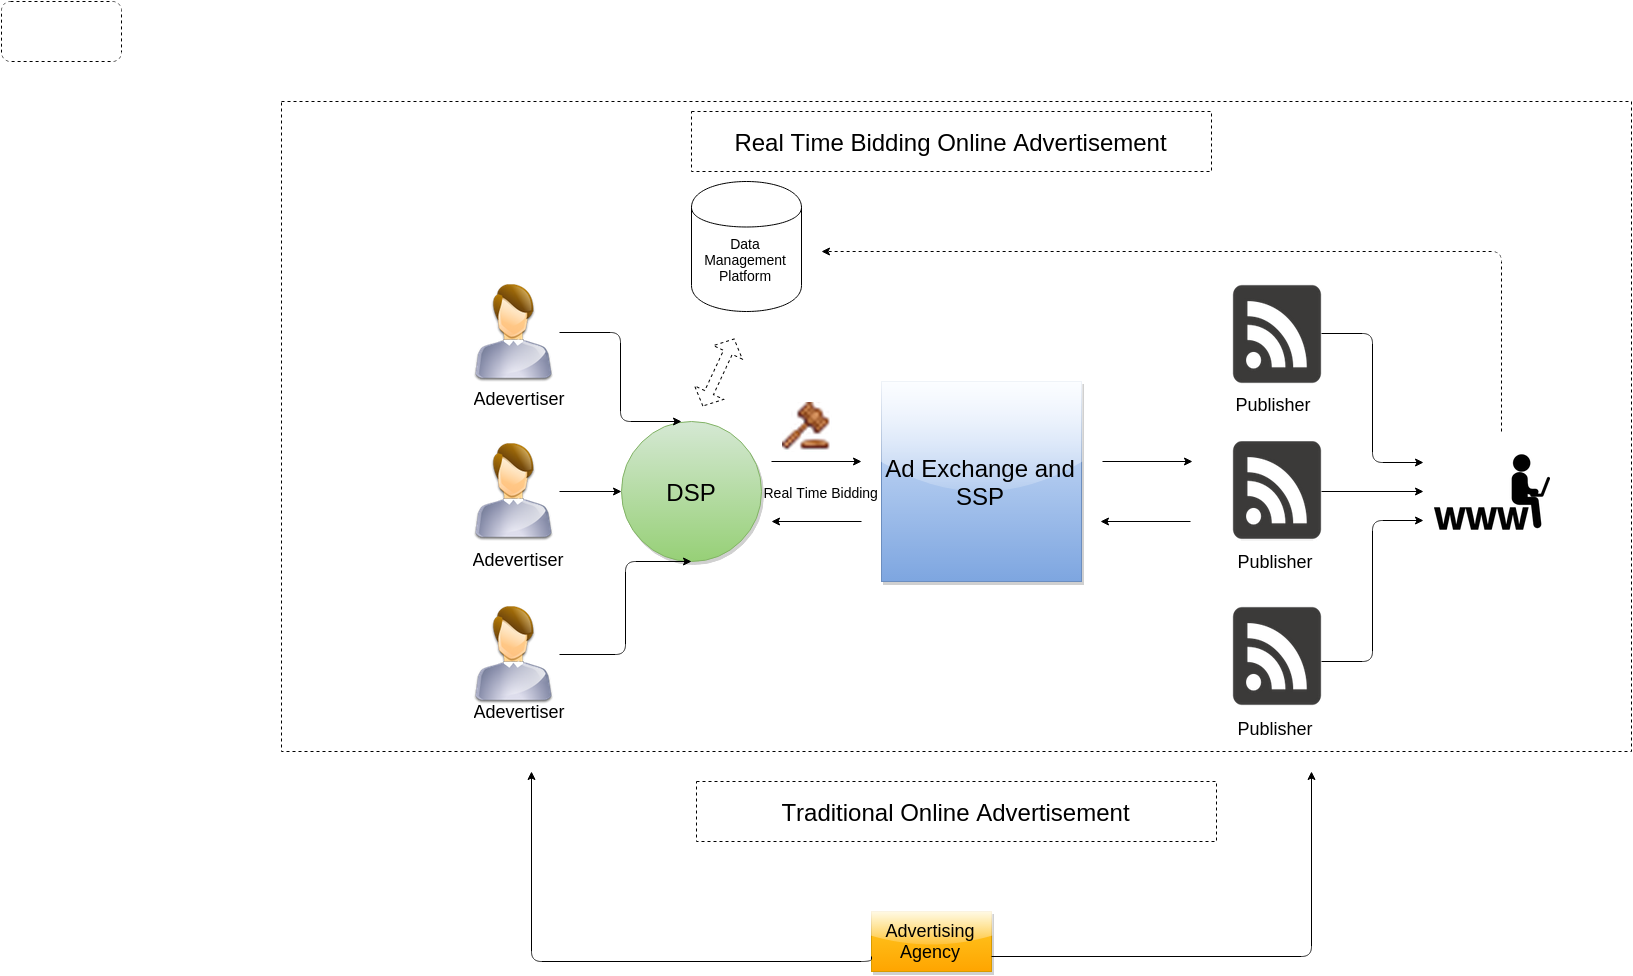
\includegraphics[width=\columnwidth]{rtblanscape.png}
\caption{Comparison between Real Time Bidding and Traditional Online Advertising}
\label{fig:ctr}
\end{figure}

\cite{cheng2012multimedia} conducts an experiment on over billions of impressions. There are also other researches on CTR prediction problem, \cite{richardson2007predicting} makes use of logistic regression to predict clicks. \cite{mcmahan2013ad} discusses on the practical engineering of CTR estimation as well as the performance of applying traditional machine learning model on complex huge dataset. \cite{zhu2010novel} discusses on General Click Model based on Bayesian network. \cite{graepel2010web} talks about \textit{Online Bayesian Probit Regression}. \cite{mohan2011web} discusses on the use of \textit{Gradient Boosting Regression Tree} (GBRT) on web ranking. GBRT algorithm is commonly used in the industry now, which is a non-linear classifier composed of a set of separators, by stacking a GBRT with LR to eliminate the non-linearity in the features it is able to give better CTR prediction results.

In conclusion, the researches on CTR are abundant for linear or non-linear regression model for sponsored search and RTB, namely how to find the \textit{right model}. However, in real industry, due to the unstructured and complex characteristic of the data, the pre-processing of data before putting into the model is more important for a real-world CTR prediction, the researches on \textit{Feature Engineering} is rare, and most of them is in the field of \textit{Natural Language Processing} (NLP), such as in \cite{garla2012ontology}, which makes use of the domain knowledge in biomedical to encode in the \textit{Unified Medical Language System} so that the machine learning clinical text classification performance can be improved largely. As said by Mohammad Pezeshki in \cite{featureengineering}

\textit{Actually the success of all Machine Learning algorithms depends on how you present the data.}

A good feature engineering means, the feature space is more flexible and easier, which means less complex model can be used but still obtain good performance, as the work in \cite{he2014practical}, the binary feature space is transformed into a lower dimension space using decision tree. Similar, in our paper, contrary to most of the researches in CTR prediction problem which focus on ML models, we will turn our focus on a more fundamental problem, namely how to prepare a better feature space for the model training.   

\section{Cold Start Problem}
The main purpose of this paper is to solve the cold start problem for CTR prediction, namely we use the data from old advertisement campaigns to predict the CTR in the new advertisement campaigns. Considering the complex and unpredictable of human behavior, this is a complicated problem. Few researches have been done to solve the cold start problem in the field of online advertising, therefore we will start to research on cold start problem in the area of \textit{recommendation system} with more abundant resources.

Cold start is a classical problem in the field of recommendation system, it focuses on the issues when the system is at the start stage without enough information so no inferences for users or items can be drew. \textit{Collaborative Filtering} (CF) is the most popular method proposed to solve this problem. In \cite{schein2002methods}, content and collaborative data are combined to solve the problem under a single probabilistic framework. \cite{su2009survey} provides a comprehensive review of collaborating filtering methods, model-based, memory-based and hybrid CF algorithms are discussed in this paper. There are also some papers focusing on solving the cold start problem based on the data itself. \cite{li2013news} proposes a personalized news recommendation model to apply ranking on hypergraph that includes users, news articles, and topics. The motivation that the researcher apply the hypergraph in news personalized recommendation is that for a news recommendation system, mining implicit relations among users, news articles, topics and named reading community is important. Given the special properties of the news articles, the researchers partition the hypergraph into multiple fine-grained 
ones, and then transform the recommendation problem into a ranking problem among the fine-grained hypergraphs. After that, the similarity graph of the news articles are built, namely setting the weights of the hyperedge. Finally, the transductive inference is performed on the news capsule in order to derive the news based on the user’s preference to provide the recommendation list for the user. \cite{jiang2012social} addresses the problem of sparsity and cold start in social recommendation. The researchers propose a \textit{Hybrid Random Walk} (HRW) algorithm to integrate multiple heterogeneous domains using signed/unsigned links,directed/undirected links and within-domain/cross-domain links into a star-structured hybrid graph in which user graph is at the center. A random walk is performed until its convergence and the steady state distribution is used for recommendation. \cite{feng2012incorporating} proposes a supervised random walk for setting of personalized tag recommendation. In this article, the heterogeneous information in the social tagging system, such as users’ tagging behaviors, tag semantics, social networks and item profiles are implemented to help alleviate the cold start problem due to data sparsity.

The above researches all focus on recommending novel items to the users based on information from heterogeneous information sources, they are not directly related to CTR prediction directly since the authors all regard data as vertex and use edge to represent the relations between the data, but we can get the insights from the literature that the information from old domains can be somewhat transformed to the new domain for the recommendation of new item. Since we can regard CTR prediction problem as a typical recommendation problem, in which advertisements with higher probability to be clicked will be recommended to the users. Therefore based on the information from the user, the advertisement itself, and the context information, we can find the position of the user profile in the network organized by these information, which confirms the certain level of generalization of the data distribution among all the domains. Therefore, it is possible to predict the CTR for new users based on the historical data as long as the logical relations exist between the historical data and the new user. 

The only paper focusing on cold start problem in the field of online advertising is \cite{agarwal2009regression}, which proposes a \textit{Regression Latent Factor} to incorporate entity features into latent factor learning. In this way the historical data and new item data can be combined together to improve the generalization of the model. We can conclude that getting the comprehensive information from history and to some point make use the new information will be a feasible way to solve the cold start problem for CTR prediction.

\section{Domain Adaptation}
In order to solve the cold start problem, we need to make use the old information in history. In the aspect of online advertising, it means how to transform the knowledge from source domains, namely old campaigns to the target domain, which is the new campaign.

The concept of domain adaptation is derived from \textit{Transfer Learning}, transfer learning is a popular research topic in the fields of artificial intelligence, machine learning, NLP, etc. In the field of machine learning, different from traditional predictive machine learning methods which ignore the difference between training and test datasets, in real world, the source and target sets should suffer from the situation of \textit{dataset shift} \cite{quionero2009dataset}, therefore, transfer learning will play a role to transfer the knowledge from current advertisement campaigns to the new ones. 

\cite{pan2010survey} makes a detailed discussion on transfer learning focusing on categorizing transfer learning for regression, classification and clustering problems. When the source and target tasks are different, and the source and target domains are same, it is called \textit{inductive transfer learning}, when the source and target domains are different however the source and target tasks are the same, it is called \textit{transductive transfer learning}. The final goal of the transfer learning system is to equip the system with the ability to recognize and apply the knowledge learned in previous domains to novel ones, which share some point of commonality. \cite{dai2007transferring} proposes a method to solve the problem of transfer learning in text classification using an EM-based naive Bayes classifier, the initial probability distribution of the source domain is estimated and then the EM algorithm is used to revise the trained model for the test dataset distribution using the unlabeled instances, this research with \cite{jiang2007instance}, \cite{huang2006correcting} and \cite{bickel2007discriminative} can be regarded as the \textit{instance based approach}. The assumption of this approach is that the source and target domains own many overlapping features, the items in the source domain will be regarded as the samples from the target domain, and part of the labeled data in the source domain can be reused in the target domain after re-weighting, the a rejection process will be made and the samples will be re-weighted again to map the target domain to the source domain to make the distributions similar. In this way, an adaptive feature representation should be developed to overcome the difference between the source and target domains. 

Another approach is \textit{feature representation transfer}, such as the researches in \cite{dai2007co}, \cite{ando2005high}, and \cite{blitzer2006domain}. In \cite{dai2007co}, a co-clustering algorithm is proposed to classify out-of-domain documents, the class label information given by the source domain can be extracted to label the word clusters for target domain. In \cite{blitzer2006domain} the domain adaptation problem in sentiment classification is discussed. No labeled data for the new domain is needed, at first \textit{N} pivot features are identified, then \textit{N} classifiers are built to predict the pivot features from remaining features, after that by computing the top eigenvectors the shared feature space can be discovered, and then the classifiers can be trained on the source domain using the augmented features. In brief, the approach of \textit{feature representation transfer} is based on the assumption that the source and target domains only share a part of the features, so the difference between the two domains can be solved by minimising the distances between the two domains, or using a multitask model to optimize the feature spaces of the two domains. In \cite{pan2011domain} the authors map the source and target domain data to the latent space spanned by the factors which can reduce domain difference and preserve original data structure. \cite{gao2008knowledge} is an example of the method \textit{parameter transfer}, which aims to discover the shared parameters or priors between the source and target domains. This approach is based on the assumption that the marginal distribution of feature space for target-domain and source-domain are similar, and also conditional probabilities also ought to be similar. In this way the parameter learned from the source domain can benefit the model for target domain. 

Our focus of this paper is to make use of transfer learning for CTR prediction problem of new advertisement campaigns. For the CTR problem, it is reasonable to say tasks between old and new campaigns are the same, which is a binary prediction classifier, however, the domains of the two will be distinct due to different data distribution and feature sets. 

From the above literature, we can make the following conclusions that we can refer to for our research. Firstly, the feature spaces of the source and target domains should be somewhat related, only if then can we transfer the knowledge learned from the source domain to the target domain, this is reasonable for the CTR problem, since even though the feature distribution from the old advertisement campaign and the new campaign can be different, the human behaviors should be related, namely the advertisements which can induce people to click should have some commonality. Secondly, the knowledge of the feature space and parameters from the model from the source domain can both benefit the CTR prediction model training in target domain. 

We also borrow the concept of \textit{domain shift} during our experiment, the comprehensive introduction of domain shift can be shown in the book \cite{quionero2009dataset}. The domain shift happens when the distribution of dataset changes arbitrarily, so the training data cannot be used directly to make predictions on the test domain. In this paper we will focus on \textit{covariate shift}, with the situation that \(Pr_{source}(x,y)\) and \(Pr_{target}(x,y)\) only differ in the marginal distribution of covariate \cite{zhang2013domain}, in the paper, we propose a machine learning method to quickly check whether the covariate shift exists between source and target datasets, ignited by the idea from \cite{coviriate}.






 











\chapter{Preliminaries}
\label{chapterlabel3}
\begin{table}[h]
\center
\vspace{-5pt}
\caption{Notations and descriptions.}
\label{tab:notation-des}
\small
\begin{tabular}{rl}
Notation & Description\\
\hline
\\ [-2.0ex]
$\bs{x_{\text{b}(N\times D)}}$ & The one-hot binary feature space.\\
$\bs{x_{\text{c}(N\times D)}}$ & The continuous counting feature space.\\
$\bs{y_{(1\times N)}}$ & The click result space\\
$w_{\text{b}(1\times D)}$ & The weights vector space of binary feature\\
$w_{\text{c}(1\times D)}$ & The weights vector space of counting feature\\
$T_{(M\times D)}$ & Transform Binary Feature to Counting Feature matrix\\
$A_{(N\times 1)}$ & Calculating frequency matrix which is an all-one vector $\vec{1 }$\\
$C_{(M\times D)}$ & Field  matrix which is a 0-1 matrix concatenated with \textsl{}{M} \\
& vectors \(V_{m,(m = 1...M)}\) and in each vector \(V_m\) only its \\
& corresponding positions in field \textsl{m} is filled with 1, \\
& with other positions 0. \\
$Diag$ & Transform the column vector into a diagonal matrix
\end{tabular}
\end{table}

\chapter{Counting Feature Theory}
\label{chapterlabel4}

\section{Introduction to Counting Feature}

RTB has dramatically transformed the display advertising industry in the last a few years \cite{yuan2013real}. Similar to stock exchanges, RTB uses algorithms to transact advertisement placements automatically for each impression real-timely. Based on context information, user history and advertisement data, the advertisements are able to be targeted to specific users thus increasing the effectiveness of display advertising as well as saving cost for advertisers. Similar to the trend that trading is transformed form paper-based to automation in financial sector, the programmatic RTB has transformed the display advertising market subversively since 2010, started in USA. Figure \ref{fig:rtbmarket} presents the huge global opportunities in RTB, the spent money will increase by 135\% from 2012 to 2017, and RTB advertisements will increase by 456\%, an annual growth rate of  40\% in the RTB advertising industry can be expected\cite{rtb2015}.

\begin{figure}[h]
\centering
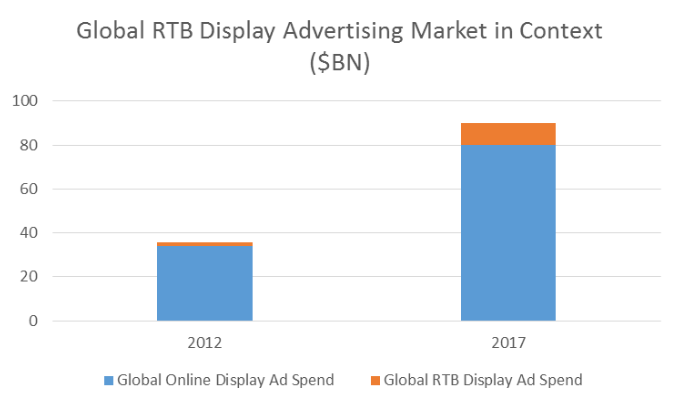
\includegraphics[width=\columnwidth]{rtbmarket.png}
\caption{Global RTB Display Advertising Market in Context}
\label{fig:rtbmarket}
\end{figure}

The core of \textit{computational advertising} is to find the \textit{optimal match} between \textit{advertisement} and \textit{users}, in some certain context \cite{balakrishnan2014real}. For the advertisers, a major concern is that whether their investments in online advertisement, like other business investments, can be paid back, namely the \textit{Return of Investment} (ROI). To specify, the profit can be represented as:\
\begin{equation}
profit = PV * CTR * ACP
\end{equation}

which is the realization formulation for sponsored search and RTB, \textit{PV} means \textit{Page View}, representing the volumes of retrieved ads, this is the upper bound of cash realization for advertising company, decided by the user experience of the recommended advertisements. \textit{CTR} means \textit{Click Through Rate}, it shows the average number of clicks for each advertisement impression, measuring the average click contribution for a single advertisement. Specifically, \textit{CTR} demonstrates the probability that one advertisement can be clicked, showing the accuracy of pushed advertisement to the audience. \textit{ACP} means \textit{Average Click Price}, which can be obtained by \(Total Cost / Total Clicks\). It is not surprising that PV, which is decide by the market share of the company and user experience, as well as ACP, which is decided by the company's strategy, are always fixed, therefore, in order to increase the ROI, predicting the CTR will be the crucial technology for advertisement and search engine companies, we can say that the CTR prediction is one of the most important part of the realization system of a company, which can be calculated by :

\begin{equation}
CTR = \frac{Clicks}{Impression} \times 100\%
\end{equation}

The key actors for CTR prediction problem can be shown in Figure \ref{fig:ctr}.

\begin{figure}[h]
\centering
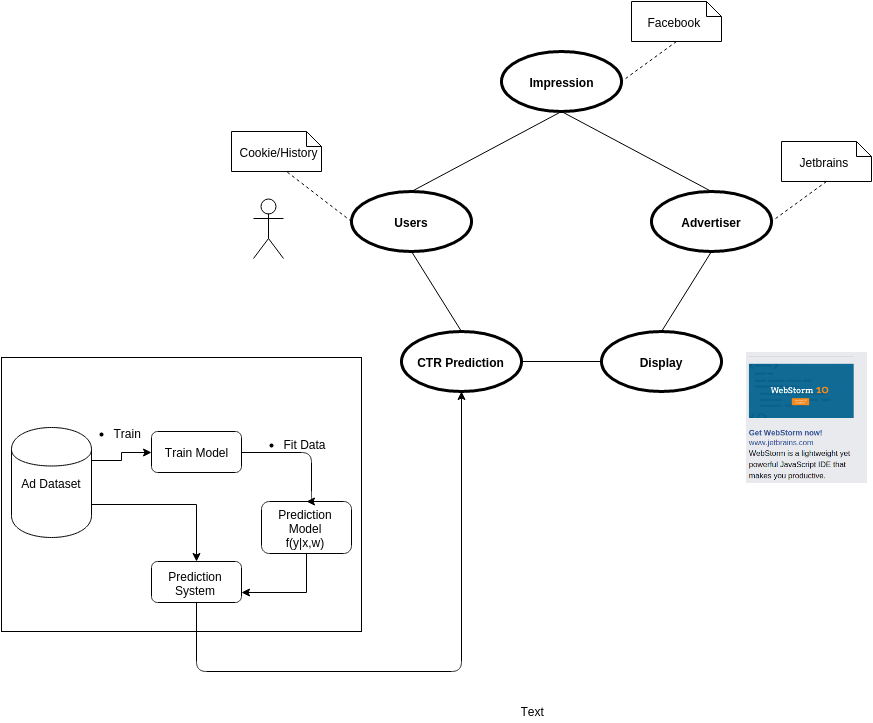
\includegraphics[width=\columnwidth]{ctr1.png}
\caption{CTR prediction Problem}
\label{fig:ctr}
\end{figure}

The challenges of the CTR prediction problem are multiple. Firstly, as we have entered the age of big data, hundreds of billions advertisements are presented every day \cite{lohr2012age}, many companies have already started the research on large-scale CTR prediction system, such as Google \cite{mcmahan2013ad}, Microsoft \cite{graepel2010web}, Baidu \cite{liu2012enlister} and Facebook \cite{he2014practical}. The problems they want to solve are similar to the challenges for big data, namely the \textit{3V} problem
\begin{itemize}
  \item Volume : With the exponential growth in the data storage for online advertisement, everyday billions of advertisements will be presented with more than a billion feature, unbalanced categories and huge data noise
  \item Velocity : The Ad data evolves a lot every second and the user behaviors change dramatically. CTR changes with time going, there are always new campaigns arising and old campaigns will expire.
  \item Variety : Advertisement data are from multiple sources, features are distinct for different campaigns, features are high dimensional and follow non-linear relations.
\end{itemize}
Therefore, the advanced online RTB advertising system must be able to handle the \textit{ZB-level, real-time} and \textit{high complexity} ad data. Models have to be trained and updated frequently and the strategies must be updated accordingly. 
The normal CTR prediction process can be represented as shown in Figure \ref{fig:system}

\begin{figure}[h]
\centering
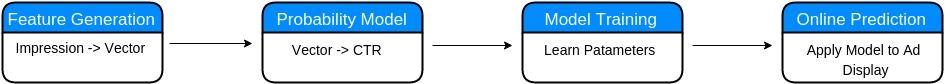
\includegraphics[width=\columnwidth]{system.png}
\caption{Machine Learning Process of CTR Prediction}
\label{fig:system}
\end{figure}

Currently, most of the researches are based on how to build a better model and algorithms, however, as said in \cite{facebook2015}, in terms of the efforts of improving the performance of ML application, the significance of the three core factors are \(Data > Features > Algorithms\). The quality of data itself and the generated features decide the upper bound of the performance of CTR prediction problem, a better algorithm and model can only help reach this upper bound as near as possible. So in this paper I will refocus on the \textit{Feature Extraction}, or \textit{Feature Engineering} which are rarely discussed but only in a few literature and blogs, such as \cite{featureengineering}, and \cite{featureengineeringmeituan}. Based on existing unstructured and complex advertisements, better generated features will help reduce the complexity of model training and relieve the \textit{cold start} problem. The new features should have the following characters:
\begin{itemize}
  \item Low Dimensionality : With the explosion of data volume, the number features will grow extremely, without feature engineering, the feature numbers will follow a linear relation with the impression number, as \(O(n)\), \(n\) is the number of impressions in the advertisement dataset. Since for giant companies, like Google or Facebook, each day more than 100 billion impressions of ad data will be generated and distributed storing on thousands machines, we can imagine the astronomical number of features which will be trained and stored, currently, one-hot features are commonly used to generate discrete binary features, for example, imagine a company owns three types of features, which are \textit{User-related},\textit{Publisher-related} and \textit{Advertiser-related}, in each type there are 10 different categories, such as \textit{region},\textit{publisher network}, \textit{advertiser network},etc. So in total there are 30 categories for each impression. For a campaign, there are 1,000,000 impressions, since the number of features equals to the number of unique items in this dataset, so according to the situation from Adform and iPinYou dataset, 5,000,000 will be a possible number of features, an impression vector will look like:
\begin{equation}
 \Big[\underbrace{[0,0,1....0,0,0]}_\textrm{Advertiser Network} + \underbrace{[0,1,0,0,0....0,0,0]}_\textrm{Publisher Network}.... \underbrace{[0,1,0,0....0,0,0]}_\textrm{Region}]
\end{equation}
Therefore, the binary one-hot feature is high dimensional and extremely sparse, and with the new come-in advertisement data, such as the ones from new campaigns, the number of features will also increase accordingly. So it is more efficient to replace the redundant and cumbersome binary feature with the feature with lower and fixed dimensions.

    \item Scalability : A huge drawback of binary feature is its lack of scalability. Imagine for Adform the old campaigns are form UK, and the CTR prediction model is trained based on the unique \textit{British Feature}, however, when a new campaign from Netherlands comes in, the overlap between the feature sets of UK old campaigns and Dutch new campaign will be small, at least the category \textit{Region} will be totally different, so the model can be only used for old campaigns and will be abandoned for new ones. Some researches have studied on how to build the model on new campaigns, but no generalized method has been proposed which is able to be used for all kinds of campaigns.
    
    \item Feature Explainability : Some companies and researchers have turned to deep learning and try to apply this magical method in the field of CTR prediction, such as the studies from \cite{deeplearning} and \cite{wang2014collaborative}, indeed, many companies now run distributed classification system for CTR prediction problems, the data training process has to be finished on Amazon EC2, but on the one hand, the method used well on one computer dose not mean that it will run perfect on distributed system, on the other hand, if deep learning is used, maybe it can improve the performance somewhat, however, firstly, it is hard to implement, secondly, the learned parameters and weights are hard to be explained , the parameters of this \textit{Black Box} cannot be interpreted with physical meanings.  
    
\end{itemize}

In order to meet the above three requirements, we propose the concept of \textit{Counting Feature}, which is totally different from the traditional \textit{Binary Feature} which is converted from categorical variables to one-hot vectors, thus sparse and mostly zeros. The counting feature essentially is a kind of \textit{statistical feature}, the one we expound is composed of \textit{Frequency Feature} and \textit{Average CTR Feature} as we discussed above. Therefore, for each categorical field in the dataset two features will be generated. For example, if we have a dataset with 3 fields, \textit{Region}, \textit{Hour}, and \textit{Cookie ID}, the the binary feature will be like: 

\begin{equation}
 \Big[\underbrace{[0,0,1....0,0,0]}_\textrm{Region} + \underbrace{[0,1,0,0,0....0,0,0]}_\textrm{Hour}.... \underbrace{[0,1,0,0....0,0,0]}_\textrm{Cookie ID}]
\end{equation}

and counting feature will be like:

\begin{equation}
 \Big[\underbrace{[0.0034,0.0001]}_\textrm{Region} + \underbrace{[0.0345,0.0002]}_\textrm{Hour}.... \underbrace{[0.0001,0]}_\textrm{Cookie ID}]
\end{equation}

Therefor counting feature can dramatically reduce the dimensionality of feature space, as shown in Figure ~\ref{fig:dimensionreduct}.

\begin{figure}[h]
\centering
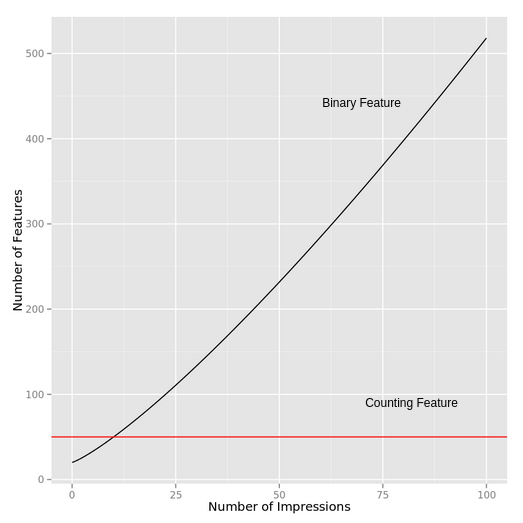
\includegraphics[scale=1.5]{dimensioncurse.png}
\caption{Dimensionality Reduction of Counting Feature}
\label{fig:dimensionreduct}
\end{figure}

Also counting feature is easy to be stretched. As we present in the \textit{Dataset Introduction} part in Chapter 5, the log data format will be the same for a certain company. The impressions is stored in the database on row-per-record basis and each field is represented in one column. Therefore, since the number of features are the same among all advertising campaigns with corresponding relations, the weights of the features learned from one campaign are feasible to be used for others, unlike binary features whose features will be unique for one campaign and cannot be scalable. 

At last, it is obvious that the parameters of the model trained using counting feature can be easily explained, for example, if the weight for the \textit{Frequency Feature} of the field \textit{Hour} is higher than the others, it means that the time when people browse the webpages play a crucial role to affect the human behavior to click on the advertisements.

One thing needed to point out here is that there are already many researches on \textit{Dimensionality Reduction}, such as \cite{burges2009dimension}, most of them are from the field of Natural Language Processing (NLP), a popular method will be Principle Component Analysis (PCA). As the method in \cite{fruergaard2013dimensionality} and \cite{dimensionreduct}, the goal of PCA is, given a \(N\) dimension space \(\mathbf{x}=(x_1,\ldots,x_n)^T\), to find a direction, namely a \(N\) dimension vector \(\mathbf{w}=(w_1,\ldots,w_n)^T\) to make sure the the linear combination \(\sum_{i=1}^nw_ix_i=\mathbf{w}^T\mathbf{x}\) can be obtained with the minimal reconstruction error or maximal characteristic. But PCA seems not applicable for the problem of CTR predtion, because:

\begin{itemize}
  \item In the PCA algorithm, firstly we need to create \(N \times d\) data matrix, in which one row vector \(x_n\) represents one data point, after subtracting the mean of \(x\) from the matrix, we need to calculate the covariance matrix of \(x\) and find eigenvectors and eigenvalues, which will take time of \(O(N*D^2)\) and memory of \(O(2*D^2)\), using SVD with another time complexity of \(O(D^3)\). Therefore it is obvious that PCA algorithm is computational intensive, especially when the number of impressions is at the level of 10 million with more than 10 million features, it is impossible to solve such a huge matrix locally. 
  \item From the view of NLP, the principle, or topics of each impression binary vector will be obtained using PCA algorithm, but unlike NLP, in the field of online advertising, we can just regard each topic as one field in the dataset, and use GBRT or other algorithms to obtain the combination of topics easily, there is no need to use PCA method.
  \item The most important thing is PCA algorithms finds the principle components by coordinate rotation, if the input feature space is not Gaussian Distribution, then the eigenvalues and eigenvectors cannot represent the characteristic of the feature distribution. It is not surprising that the sparse binary feature space does not follow a normal distribution, so PCA is not applicable here. 
\end{itemize}

Therefore, we believe counting feature is the only feature space to satisfy the above three requirements and we will discuss on its properties and performance in the rest of the paper. 


\section{Relation Between Counting Feature and Binary Feature}
In this section we will present the deduction of the relation between \textit{Counting Feature} and \textit{Binary Feature} in the context of \textit{Linear Regression Model}, in the field of online advertising, each data porint is \(Impression = \{ x_i,y_i \}_{1 \leq i \leq N}\)  where each \(x_i  \in \mathbb{R}^n\) and \(y_i \in \mathbb{R}\), and \(N\) is the number of impressions in the dataset, \(x\) is the feature space and \(y\) is the click label. Assuming that the click label follows the basic linear relation with feature space, as follows:
\begin{equation}
y_i =w_0 +\sum_j w_j x_{ij} =w_0 +w^T x_i 
\end{equation}
By redefining \(x_i = (1,x_i)\) and combining \(w_0\) and \(w_i‘s\) into a single weights vector we can get 
\begin{equation}
y_ i = w^T x_i 
\end{equation}

According to \cite{prince2012computer} and use \textit{Maximum Likelihood Estimation} method, the click label \(y_i\) can be assumed to have Gaussian noise error, \begin{equation}
y_i = w^T x_i + \epsilon 
\end{equation}
where \(\epsilon \sim N(0,\sigma^2)\).
Then the likelihood can be obtained by :
\begin{equation}
\mathcal{L}(D | w, \sigma) = (2 \pi \sigma^2)^{-n/2} \prod_{i=1}^{n} exp \left[ \frac{-(y_i - \hat{y}_i)^2}{2\sigma^2} \right] 
\end{equation}
and 
\begin{equation}
w_{MLE} = argmin_w \sum_i  (y_i - w^T x_i)^2 
\end{equation}
At last we can obtain that 
\begin{equation}\label{eq:w}
\hat{W} = (X^T X)^{-1} X^T Y 
\end{equation}
in which  \(X = (x_1, x_2, \ldots, x_N)^T\), \(Y = (y_1, y_2, \ldots, y_N)^T\) and \(W = (w_0, w_1, w_2, \ldots, w_N)^T\)

In the rest of this section, we will demonstrate how to transform the weight space of binary feature to that of \textit{Frequency Feature} and \textit{Average CTR Feature} respectively, the notation used in the math equations in the rest of the section is shown in Table \ref{tab:notation-des}
\begin{table}[h]
\center
\vspace{-5pt}
\caption{Notations and descriptions.}
\label{tab:notation-des}
\small
\begin{tabular}{rl}
Notation & Description\\
\hline
\\ [-2.0ex]
$\bs{x_{\text{b}(N\times D)}}$ & The one-hot binary feature space.\\
$\bs{x_{\text{c}(N\times D)}}$ & The continuous counting feature space.\\
$\bs{y_{(1\times N)}}$ & The click result space\\
$w_{\text{b}(1\times D)}$ & The weights vector space of binary feature\\
$w_{\text{c}(1\times D)}$ & The weights vector space of counting feature\\
$T_{(M\times D)}$ & Transform Binary Feature to Counting Feature matrix\\
$A_{(N\times 1)}$ & Calculating frequency matrix which is an all-one vector $\vec{1 }$\\
$C_{(M\times D)}$ & Field  matrix which is a 0-1 matrix concatenated with \textsl{}{M} \\
& vectors \(V_{m,(m = 1...M)}\) and in each vector \(V_m\) only its \\
& corresponding positions in field \textsl{m} is filled with 1, \\
& with other positions 0. \\
$Diag$ & Transform the column vector into a diagonal matrix
\end{tabular}
\end{table}


\subsection{Frequency Feature}

The CTR predictino problem can be regarded as a classical classification problem in Machine Learning, we can use features of ads, terms, and advertisers to learn a model that accurately predicts the CTR for new ads. The training dataset contains a number of \textsl{N} instances, which are the records in datalog containing \textsl{M} fields of user, advertiser and publisher information, as well as their click label for each ad impression. The result of the impression, namely whether the user clicks on the ad will be represent by \textsl{y}. Since here the dependent variable is dichotomous, the liner regression can be used to prove the relation between model built by \(x_{\text{c}}\) representing the data instances encoded into \textsl{Counting Feature} and model built by \(x_{\text{b}}\) representing the data instances encoded into one-hot \textsl{Binary Feature}. The dimension of the \textit{frequency feature} and \textit{average CTR feature} is the number of fields \textsl{M} well the dimension of \(x_{\text{binary}}\) is represend by \textsl{D} for which \(D >> M\). The more detailed information about symbols are shown in Table 3.1.
\iffalse
\begin{itemize}
\item  Binary Features : \(x_{\text{binary}(N\times D)}\)
\item  Counting Feature : \(x_{\text{counting}(N\times D)}\)
\item  Clicking result : \(y_{(1\times N)}\)
\item  Weights vector of Binary Feature : \(w_{\text{binary}(1\times D)}\)
\item  Weights vector of Counting Feature: \(w_{\text{counting}(1\times M)}\)
\item  Transform Binary Feature to Counting Feature matrix : \(T_{(M\times D)}\)
\item  Calculating feaquency matrix : \(A_{(N\times 1)}\) which is an all-one vector 
$\vec{1 }$  
\item  Field  matrix : \(C_{(M\times D)}\) which is a 0-1 matrix concatenated with \textsl{}{M} vectors \(V_{m,(m = 1...M)}\) and in each vector \(V_m\) only its corresponding positions in field \textsl{m} is filled with 1, with other positions 0.
\item  Diag function : Transform the column vector into a diagonal matrix.\vspace{5mm} 

\end{itemize}
\fi
 It can be proven that 
\[ T = C\times Diag(x_{b}A) \]
The formation of \textsl{T} is 

$$
\begin{pmatrix} 
\vec{F_1} \\
\vec{F_2} \\
.\\
\vec{F_M}

\end{pmatrix}
$$

\noindent in which \($$\vec{F_m}$$ = $$\begin{pmatrix} 
$$\vec{0 }$$ , f_{m1}, f_{m2}, ...f_{mi}... , f_{mI} ,$$\vec{0 }$$ 
\end{pmatrix}$$\), and \(f_{mi}\) represents the occurrence of \(i_{th}\) binary feature in the field \textsl{m} in the whole dataset.\vspace{5mm}

\noindent Next, the relations between \(w_{\text{binary}}\) and \(w_{\text{counting}}\) are proven as follows. 

\begin{equation}
w_{\text{b}} \times x_{\text{b}}^T = y 
\end{equation}

\begin{equation}
(w_{\text{b}}^T \times w_{\text{b}}) \times x_{\text{b}}^T = w_{\text{b}}^T \times y 
\end{equation}

\begin{equation}
x_{\text{b}}^T = (w_{\text{b}}^T \times w_{\text{b}})^{-1} \times w_{\text{b}}^T \times y 
\end{equation}

Using SVD, we can derive that,

\begin{equation}
(w_{\text{b}}^T \times w_{\text{b}})^{-1} \times w_{\text{b}}^T = (w_{\text{b}})^{-1(left)}  
\end{equation}

So we can get that 
\begin{equation}
x_{\text{b}}^T =  (w_{\text{b}})^{-1(left)} \times y 
\end{equation}

We define
\begin{equation}
T = C \times Diag(x_{\text{b}}^T \times A)
\end{equation}


Multiply each size by \textsl{T}, we can get
 
\begin{equation}
T \times x_{\text{b}}^T =  T \times (w_{\text{b}})^{-1(left)} \times y 
\end{equation}

It can be proven that 
\begin{equation}
T \times x_{\text{b}}^T =  x_{\text{c}}
\end{equation}

So
\begin{equation}
x_{\text{c}} =  T \times (w_{\text{b}})^{-1(left)} \times y 
\end{equation}

Since \(T \times (w_{\text{b}})^{-1(left)}\) is a \(M \times 1\) matrix, so multiplying its transposition we can get a constant scalar, 
\begin{equation}
(T \times (w_{\text{b}})^{-1(left)})^T \times (T \times (w_{\text{b}})^{-1(left)}) = \lambda
\end{equation}

So, 
\begin{equation}
1/{\lambda} \times (T \times (w_{\text{b}})^{-1(left)})^T \times x_{\text{c}} =  y
\end{equation}

In conclusion, we can get
\begin{equation} \label{eq:12}
\begin{split}
w_{\text{c}} & =\ 1/{\lambda} \times (T \times (w_{\text{b}})^{-1(left)})^T \\
& = \ 1/{\lambda} \times (C \times Diag(x_{\text{b}}^T \times A) \times (w_{\text{b}})^{-1(left)})^T
\end{split}
\end{equation}

substitute \(W\) with \((X^T X)^{-1} X^T Y\), we can get:
\begin{equation} \label{eq:13}
\begin{split}
w_{\text{c}} & =\ 1/{\lambda} \times (T \times (w_{\text{b}})^{-1(left)})^T \\
& = \ 1/{\lambda} \times (C \times Diag(x_{\text{b}}^T \times A) \times ((x_{\text{b}}^T x_{\text{b}})^{-1} x_{\text{b}}^T y)^{-1(left)})^T
\end{split}
\end{equation}

\subsection{Average CTR feature}

\setlength{\parindent}{5ex}

In this section, the relation between  \(w_{\text{ctr}}\) and \(w_{\text{binary}}\) will be deduced, the steps are similar except for specific part of CTR calculating. 

Initially, we can get the similar deduction process, 
\begin{equation}
w_{\text{b}} \times x_{\text{b}}^T = y 
\end{equation}

\begin{equation}
(w_{\text{b}}^T \times w_{\text{b}}) \times x_{\text{b}}^T = w_{\text{b}}^T \times y 
\end{equation}

\begin{equation}
x_{\text{b}}^T = (w_{\text{b}}^T \times w_{\text{b}})^{-1} \times w_{\text{b}}^T \times y 
\end{equation}

\begin{equation}
(w_{\text{b}}^T \times w_{\text{b}})^{-1} \times w_{\text{b}}^T = (w_{\text{b}})^{-1(left)}  
\end{equation}

\begin{equation}
x_{\text{b}}^T =  (w_{\text{b}})^{-1(left)} \times y 
\end{equation}

However, then in order to count the number of \textsl{clicks} for each instance, we redefine the transformation matrix \textsl{T} as following, 

\begin{equation}
T_{\text{click}} = C \times Diag(x_{\text{b}}^T \times y)
\end{equation}



From section 1, we can know that, 
\begin{equation}
T_{\text{frequency}} = C \times Diag(x_{\text{b}}^T \times A)
\end{equation}

Since it is easy to know that,

\begin{equation}
(Diag(T_{\text{click}}) \times (1/T_{\text{frequency}} )^T =  T_{\text{ctr}}
\end{equation}

Similar to section 1, we can multiply \(T_{\text{ctr}}\) by both sides of equation (17)

\begin{equation}
T_{\text{ctr}} \times x_{\text{b}}^T =  T_{\text{ctr}} \times (w_{\text{b}})^{-1(left)} \times y 
\end{equation}

It can be proven that 

\begin{equation}
T_{\text{ctr}} \times x_{\text{b}}^T =  x_{\text{ctr}}
\end{equation}

So,

\begin{equation}
 x_{\text{ctr}} =  T_{\text{ctr}} \times (w_{\text{b}})^{-1(left)} \times y 
\end{equation}

It is similar to section 1 that \(T_{\text{ctr}} \times (w_{\text{binary}})^{-1(left)}\)is a \(M \times 1\) matrix, so we define, 
\begin{equation}
(T_{\text{ctr}} \times (w_{\text{b}})^{-1(left)})^T \times (T_{\text{ctr}} \times (w_{\text{b}})^{-1(left)}) = \lambda
\end{equation}

So, 
\begin{equation}
1/{\lambda} \times (T_{\text{ctr}} \times (w_{\text{b}})^{-1(left)})^T \times x_{\text{ctr}} =  y
\end{equation}

In conclusion, we can get
\begin{equation} 
\begin{split}
w_{\text{ctr}} & =\ 1/{\lambda} \times (T_{\text{ctr}} \times (w_{\text{b}})^{-1(left)})^T \\
& = \ 1/{\lambda} \times (Diag(T_{\text{click}}) \times (1/T_{\text{frequency}} )^T \\ 
& \times (w_{\text{b}})^{-1(left)})^T \\
& = \ 1/{\lambda} \times (Diag(C \times Diag(x_{\text{b}}^T \times y)) \\ 
& \times (1/ (C \times Diag(x_{\text{b}}^T \times A) )^T) \times (w_{\text{b}})^{-1(left)})^T
\end{split}
\end{equation}
and
\begin{equation} 
\begin{split}
w_{\text{ctr}} & =\ 1/{\lambda} \times (T_{\text{ctr}} \times (w_{\text{b}})^{-1(left)})^T \\
& = \ 1/{\lambda} \times (Diag(T_{\text{click}}) \times (1/T_{\text{frequency}} )^T \\ 
& \times (w_{\text{b}})^{-1(left)})^T \\
& = \ 1/{\lambda} \times (Diag(C \times Diag(x_{\text{b}}^T \times y)) \\ 
& \times (1/ (C \times Diag(x_{\text{b}}^T \times A) )^T) \times ((x_{\text{b}}^T x_{\text{b}})^{-1} x_{\text{b}}^T y)^{-1(left)})^T
\end{split}
\end{equation}

\subsection{Non-linearity of Counting Feature}
From the above deduction, we can draw the conclusions that
\begin{itemize}
\item The transformation matrix can help transform the high-dimension binary feature space into low-dimension counting feature space, which is a non-linear transformation.
\imte The weight space of binary feature model can be transformed into that of counting feature model in a non-linear way.
\end{itemize}
In the following of the paper, we will use \textit{logistic regression} which is a popular discriminative classifier to directly learn \(P(Y|X)\) and model the binary class boundary for \textit{Binary Feature}, as follows:
\begin{equation}
P(Y = 1| X) = \frac{exp(w_{0} + \sum_{i = 1}^{n} w_{i}x_{i})}{1 + \exp(w_{0} + \sum_{i = 1}^{n} w_{i}x_{i})}  
\end{equation}
and 
\begin{equation}
P(Y = 0| X) = \frac{1}{1 + \exp(w_{0} + \sum_{i = 1}^{n} w_{i}x_{i})}  
\end{equation}
The precondition of using logistic regression is that the dependant features and the target (click) follow the linear regression, since we already know that the \textit{counting feature} is a non-linear transformation of \textit{binary feature}, we can define the non-linear formulation of logistic regression as follows:
\begin{equation}
Pr(w_{\text{i}}|x_{\text{i}}) = Bern_{w_{\text{i}}}[sig(a_{\text{i}})]
\end{equation} \cite{prince2012computer}

in which \(sig(a_{\text{i}})\) is the sigmoid function and the activation \(a_{\text{i}}\) is given by,

\begin{equation}
a_{\text{i}} = \Phi^T f(x_{\text{i}})
\end{equation}

The function and \(f(x)\) is the nonlinear transformation of the space \(x\), \(f(x_{\text{i}})\) can be represented as \(T x_{\text{b}}^T \) in terms of \textit{Frequency Feature} (Average CTR Feature has a similar relation), that is:
\begin{equation}
f(x_j) = \sum_{i=1}^{D}T_{ji} x_\text{b}_i  
\end{equation}
in which \(j\) is the \(j_th\) field of the dataset and \(i\) is the \(i_th\) dimension of binary feature. 

In our case of frequency feature and average CTR feature, the weights space should be derived as \(\Phi^T \) using incremental fitting and boosting model. 

%So we successfully transform the linear logistic regression on \(N\) dimension to the incremental fitting and boosting problem, we will do some experiment to prove the equivalence of them.

\begin{figure}[h]
\centering
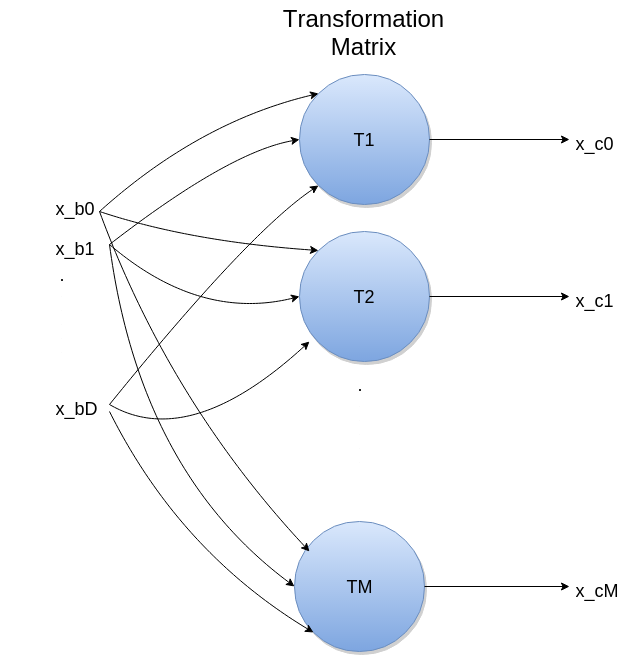
\includegraphics[scale = 1.5]{countingfeature.png}
\caption{Binary Feature to Counting Feature}
\label{fig:counting}
\end{figure}
In summary, we can see \textit{counting feature} as a nonlinear transformation from \textit{binary feature} from the same dataset, which can be seen as a statistical representation of binary feature, compressing the information of the whole dataset. Counting feature can reduce the high dimension of binary feature to lower dimensions, namely from millions of dimensions to less than 1 hundred. The cost of this reduction is assuming that binary feature follows a linear model to the label, such a space transformation will lead to the non-linearity of the counting feature. So we have to use non-linear regression model, such as Gradient Boosting Decision Decision (GBDT) to solve this problem. Using the method in \cite{he2014practical}, one way to do so is to transform the input space so that the non-linearity is eliminated and a linear feature space can be obtained, this can be done by GBDT, and according to \cite{cover1965geometrical}:

\textit{"A complex pattern-classification problem, cast in a high-dimensional space nonlinearly, is more likely to be linearly separable than in a low-dimensional space, provided that the space is not densely populated."}

So the counting feature can be trained into the model when following a non-linear regression model to eliminate the non-linearity meanwhile obtain the comparable performance in terms of CTR prediction with binary feature.

In Chapter 5.2, we will show the performance comparison of binary feature and counting feature in the context of real world online advertising dataset from Adform using both Logistic Regression Model and GBDT model. 
The logistic regression model is:
\begin{equation}
CTR = P(Y|X,w) = \frac{1}{1 + \exp(-a)}  
\end{equation}
In which \(a = \phi^T x\)

Using the training dataset \((x_i,y_i)\), and using \(L_\text{1}\) regularization, we can get the loss function as:
\begin{equation}  \label{eq:object}
min_w \sum_{i}^{N} [y_i In(1+\exp {-w^T x_i}) + (1-y_i) In(1+\exp {w^T x_i})] + c||w||_1, ||w|| = \sum_j=1^D |w_j|
\end{equation}

And we will use Newton Method to solve the problem, the gradient ascent computes the most optimal parameters by updating in the direction of gradient iteratively as 
\begin{equation}
w_{i} \rightarrow w_{i} + \alpha \frac{\partial l(w)}{\partial w_{i}}  
\end{equation}
where 
\begin{equation}
\frac{\partial l(w)}{\partial w_{i}} = \sum_{t} X^{t}_{i}(Y^{t} - \hat{P}(Y^{t} = 1|X^{t}, w))  
\end{equation}

As for GBDT algorithm, referring to the method in \cite{boostedtree}, we will use the idea of \textit{boosted trees} to realize the non-linear logistic CTR prediction model. The objective function of GBDT can be regarded as the same as \ref{eq:object}, the tree ensemble model is used here which is the \textit{classification and regression trees} (CART). For each classification tree we can obtain a score for the prediction task, the sum up of the scores from individual tree will lead to the final score of prediction. The model can be fomulated as:
\begin{equation}
y_i = \sum_{k=1}^K f_k(x_i), f_k \in F
\end{equation}
where \(K\) is the number of trees, and \(f\) is a function in the functional space of all possible CARTs. Using the method of \textit{Additive Training} the objective method can be solved and the parameters of the trees can be obtained. The details of the GBDT method can be referred in \cite{boostedtree} and \cite{he2014practical}.

The comparison results show that the performance of counting feature using non-linear regression model (GBDT) is comparable to that of binary feature using linear regression model (Logistic regression model), using Area under the curve (AUC) as the criteria, which proves the correctness and retionality of counting feature.

\section{Counting Feature Generalization}
In this part, we will briefly discuss on the generalization of counting feature, to prepare for the next chapter. Our assumption is that counting feature has a better property of generalization than binary feature, we have the following backup which is considered in terms of weight space of the CTR prediction models.
We will compare the weight space of binary and counting feature, from \ref{eq:12} we can get the following equation:
\begin{equation} \label{eq:28}
\begin{split}
w_{\text{counting}} & =\ 1/{\lambda} \times (C \times Diag(x_{\text{binary}}^T \times A) \times (w_{\text{binary}})^{-1(left)})^T \\
& = \ 1/{\lambda} \times (C \times Diag(x_{\text{binary}}^T \times A) \times ((w_{\text{binary}}^T \times w_{\text{binary}})^{-1} \\
& \times w_{\text{binary}}^T )^T
\end{split}
\end{equation} 

It is obvious that the dimension of counting feature is much less than binary feature. Imagine we have two campaigns from each we can obtain the weight space using logistic regression model, which are \(w_1\) and \(w_2\). Mathematically, we know that in the space the included angle \(\theta\) of two vectors in \(n\) dimension follow the probability density function of 

\begin{equation}
p(\theta)=\frac{\Gamma(\frac{n}{2})}{\Gamma(\frac{n-1}{2})}
\frac{\sin^{n-2}(\theta)}{\sqrt\pi}
\end{equation}

Therefore in a high dimension the two vectors will be almost vertical to each other, which means the weight space of binary features for two campaigns will be uncorrelated to each other

In Figure \ref{fig:three graphs}, using the top 10 campaigns from Adform dataset which is introduced in detail in Chapter 5, we do the experiment as follows,
\begin{enumerate}
\item we train the CTR prediction model using logistic regression model for each campaign in terms of counting feature and binary feature, to obtain \([w_{b1},w_{b2},...w_{b10}]\), and \([w_{c1},w_{c2},...w_{c10}]\)
\item Then for the 10 binary weight spaces and counting weight spaces, we calculate the cos similarity, correlation, and euclidean distance for each pair of the weights space
\end{enumerate}
 
The result is shown in Figure \ref{fig:three graphs} from which we can see the weight space of counting feature are much more similar to each other than that among binary features.
\begin{figure}[h]
    \centering
    \begin{subfigure}{0.3\textwidth}
        \includegraphics[width=\textwidth]{cos}
        \caption{Cos Similarity Comparison Between Pairwise of Binary Feature and Counting Feature}
        \label{fig:cos}
    \end{subfigure}
    \hfill
    \begin{subfigure}{0.3\textwidth}
        \includegraphics[width=\textwidth]{correlation}
        \caption{Correlation Similarity Comparison Between Pairwise of Binary Feature and Counting Feature}
        \label{fig:correlation}
    \end{subfigure}
    \hfill
    \begin{subfigure}{0.3\textwidth}
        \includegraphics[width=\textwidth]{euclidean}
        \caption{Euclidean Distance Comparison Between Pairwise of Binary Feature and Counting Feature}
        \label{fig:euclidean}
    \end{subfigure}
    \caption{Comparison of Binary and Counting Feature Model Weights Space}
    \label{fig:three graphs}
\end{figure}
%Now the experiment is done in which the placement id is counted and when the clicks in one palcement id's corresponding is higher than 200, the instances will be remained, and the overlap of placement id in the train dataset and test dataset will be filtered out. Then for the training dataset all the campains in the test dataset are new. Many experiments are done now but result is confused. Generally the result is as follows: 

From Figure \ref{fig:three graphs} it shows the similarities among weight spaces of counting feature are significantly higher than that of binary feature, and weight spaces of binary feature are hardly related.  Therefore, we can say that since the counting values are continuous ranging from 0 to 1, the variability of data distribution among different campaigns are largely transformed from weight space to feature space for counting feature. Even though directly using the weight space trained from old campaign to new campaign will lead to poor performance initially for both counting feature and binary feature, with the income new data containing the information of distribution from new campaign, we are able to update the values of counting feature to force the model trained from the old campaign to be \textit{alike} the new campaign, however for binary feature the variability of the model is taken by the weight space since there are only 0 and 1 for the binary feature value, so it is not possible to transform the statistical information from new campaign to the old model. 

So it is reasonable to presume that counting feature can be used to alleviate the cold start problem.

\iffalse
I am trying to figure out the reason why binary feature performs well in cold start problem and it seems biased dataset is a cause and I try to split the model into generic and specific parts and overcome the bias.
\subsection{Model Similarity Analysis}
At first, we will start from the easier one, the frequency feature. Let's assume that we have two datasets, dataset \(Dataset_{\text{1}}\) and \(Dataset_{\text{2}}\), for each dataset we can get \(w_{\text{counting}}\) and \(w_{\text{binary}}\) respectively. Let's abbreviate them as \(w_{\text{c1}}\) and \(w_{\text{b1}}\) as well as \(w_{\text{c2}}\) and \(w_{\text{b2}}\). 

From \ref{eq:12} we can get the following equation:
\begin{equation} \label{eq:28}
\begin{split}
w_{\text{counting}} & =\ 1/{\lambda} \times (C \times Diag(x_{\text{binary}}^T \times A) \times (w_{\text{binary}})^{-1(left)})^T \\
& = \ 1/{\lambda} \times (C \times Diag(x_{\text{binary}}^T \times A) \times ((w_{\text{binary}}^T \times w_{\text{binary}})^{-1} \\
& \times w_{\text{binary}}^T )^T
\end{split}
\end{equation}

We will make use of cos similarity, which is used to measure the distance between two vectors to measure the similarity of two \(w_{\text{counting}}\) from \(Dataset_{\text{1}}\) and \(Dataset_{\text{2}}\). The formation of similarity can be shown as follows:

\begin{equation} \label{29} 
\begin{split}
Similarity & = \cos(\Theta) = \frac{w_{\text{c1}} \times w_{\text{c2}}^T} {||w_{\text{c1}}|| \times ||w_{\text{c2}}|| }
\end{split}
\end{equation}

Substitute \(w_{\text{c1}}\) with \ref{eq:12} and represent \(Diag(x_{\text{binary}}^T \times A)\) using \(Diag(f)\) since this diagonal entries \(d(i,i) \) shows the frequency of feature \(i\), we can get the following equation:


\begin{equation} \label{30} 
\begin{split}
\frac{w_{\text{c1}} \times w_{\text{c2}}^T} {||w_{\text{c1}}|| \times ||w_{\text{c2}}|| } & =  \frac{w_{\text{c1}} \times w_{\text{c2}}^T} {\sqrt{w_{\text{c1}} \times w_{\text{c1}}^T} \times \sqrt{w_{\text{c1}} \times w_{\text{c2}}^T} }
\end{split}
\end{equation}

To simply, at first we will deduct the following equation:

\begin{equation} \label{31} 
\begin{split}
w_{\text{ci}} \times w_{\text{cj}}^T & = \frac{1}{{\lambda}_{i}{\lambda}_{j} } \times (w_{\text{bi}} \times Trans_{i}) \times (w_{\text{bj}} \times Trans_{j})^T \\
& subject : (i.j = 1 \cup 2)
\end{split}
\end{equation}

\fi
%In which \(Trans\) is a Transformation Matrix, 
%\begin{equation} \label{31} 
%\begin{split}
%Trans = ((w_{\text{binary}}^T \times w_{\text{binary}})^{-1})^T \times (Diag(f))^T \times C^T  
%\end{split}
%\end{equation}

%Then, we will focus on the transformation matrix. 

%Since \(((w_{\text{binary}}^T \times w_{\text{binary}})^{-1})^T\) is a symmetric matrix, so it equals to its own transposition. 



\chapter{Cross Domain Learning For Online Advertisement}
\label{chapterlabel5}
\section{Domain Adaptation and Transfer Learning}
Traditional supervised learning is relied on the assumption that the distribution of training and test instances are similar. However, it is rare in real life that the distributions among datasets are unchanged. As discussed in \cite{facebook2015}, many proposed machine learning algorithms and models can be only used under the assumption that the training and test datasets are derived from the same distribution and with same feature space, when the distribution changes, new data needs to be collected and new model needs to be rebuilt. For the industry of online advertisement, it is expensive time-consuming to rebuild the model, in this case, transfer learning is needed which can borrow the knowledge learned from previous advertisement campaigns and apply to new campaigns to increase the efficiency for CTR prediction and decrease the cost for training new model. Although now directly related but similar to the research in \cite{pan2008transfer}, the behaviors of users among different campaigns are volatile and unpredictable, in traditional statistical machine learning problem, it is based on the ideal assumption that the model learned will not affect the real world, independent and identically distributed samples on different campaigns ensures the generalization. However when it comes to the real-world online advertisement industry, after the model is introduced into production, the users behavior will be affected, and also the distribution of the data. In brief, the changeable user behaviors among online advertisement campaigns determines that static statistical model is not suitable for dynamic online advertisement CTR prediction, \textit{transfer learning} is desirable which can save significant time and effort. 


\begin{figure}[t]
\centering
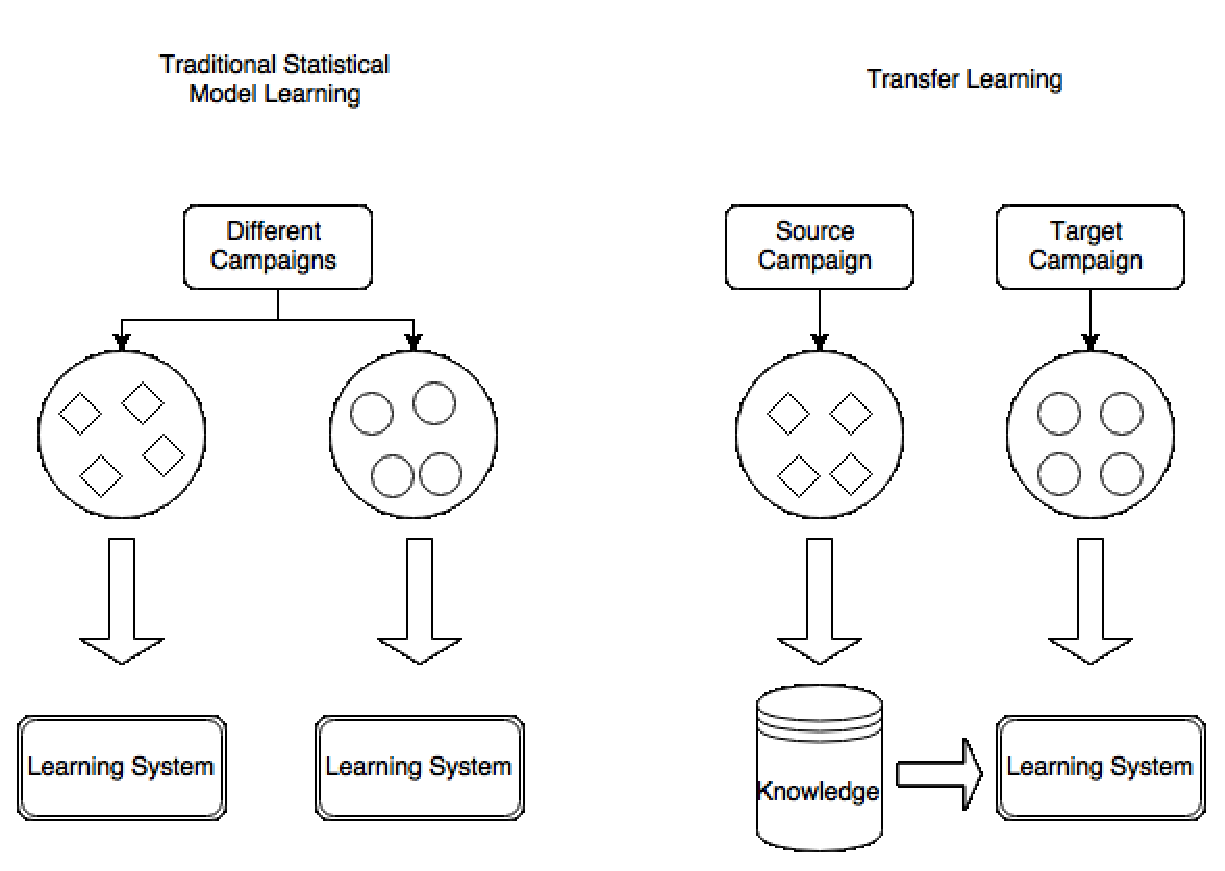
\includegraphics[width=\columnwidth]{transferlearning.eps}
\caption{Different Learning system between traditional machine learning and transfer learning}
\label{fig:transfer}
\end{figure}

At first, using the definitions in \cite{pan2010survey}, we specify \textit{domain} \textit{D} as each campaign's impressions raw data, and \textit{task} \textit{T} as the learning system of the model, in which, \(D = \{X,P(X)\}\), also  \(D = \{Y,P(Y|X)\}\). \(X = \{x_1,x_2, ..., x_n\}\) in which \(x_i\) is one impression in the campaign, and \(Y = \{y_1,y_2, ..., y_n\}\) is the label for each impression, namely whether in this impression the click occurs. The training data is composed of the pairs of \(\{x_i,y_i\}\) which can be used to train the model, and the conditional distribution \(P(Y|X)\). We define \textit{source domain} as the old campaign and \textit{target domain} as the new campaign, then \(X_s\) will be the feature space of source domain and \(P(X_s)\) is the marginal probability distribution of the feature space of source domain, similar, \(X_t\) will be the feature space of target domain and \(P(X_t)\) is the marginal probability distribution of the feature space of target domain. \(Y_s\) is the class label of the features in source domain and \(Y_t\) will be the corresponding label for target domain. By considering the relation between source domain and target domain, as well as source task and target task, the model learning problem can be classified as follows in the scope of online advertisement. 

\begin{enumerate}
\item if \(D_s = D_t\) and \(T_s = T_t\), this is a traditional machine learning problem. For example, the source and target advertisement campaigns follow the same distribution, and their learning tasks are the same, which are to predict the CTR based on the feature spaces. 

\item if  \(D_s \neq D_t\) and \(T_s = T_t\), which means the source and target domains are distinct but with the same tasks. The problem is also known as \textit{domain adaptation} \cite{arnold2007comparative} since the two domains are different in the marginal probability distribution but same for tasks. This situation can be further classified into two types:
    \begin{itemize}
    \item  \(X_s \neq X_t\), which means the feature spaces of the two domains are different with each other, for example, one domain of an advertisement campaign  \textit{International e-commerce} and the other is from \textit{ Software} as shown in \cite{zhang2014real}, if the impressions of the two domains are encoded into binary feature, surely there will be small overlap between the two feature spaces and the feature spaces will be largely different.
    \item \(P(X_s) \neq P(x_t) \), which means the probability distributions of the two advertisement campaigns are different, so they are from different fields, with different themes. 
    
    \end{itemize}
\item if  \(D_s = D_t\) and \(T_s \neq T_t\), it can also be classified into two types:
     \begin{itemize}
    \item  \(Y_s \neq Y_t\), this means the label spaces are different for two domains, as an example for online advertisement, the label in one domain could be click/non-click, which is dichotomic, but in the other domain the labels can be winning price, which is continuous.
    \item \(P(Y_s|X_s) \neq P(Y_t|X_t) \), this means the conditional probability distributions of the label on feature spaces are different for two domains, one example can be due to the existence of online robots, for one campaign all the impressions are randomly clicked or seen by programs, but the other campaign successfully prevent themselves from the robots so all clicks are effective and valid which simulates the human behaviors in the real world.  
  \end{itemize}
\end{enumerate}

In this paper, we will focus on transductive transfer learning, or \textit{domain adaptation}, since our learning task is obvious, which is CTR prediction, and we assumes that the robots are rare in the campaign, so the conditional probability are similar between the two campaigns, since the similar human behaviors will lead to similar advertisement clicking actions. 

As discussed above, domain is composed of feature space and feature probability distribution. In this paper, since our goal is to compare the performance of binary feature and counting feature, so we will represent the feature space and feature probability distribution of source and target domain in Table~\ref{tab:domainadapt}.

\begin{table}[t]
\begin{tabular}{ c | l | l }
Feature Types & Feature Space & Feature Distribution \\
\hline \hline
Binary Feature & Different & Different  \\
Counting Feature & Same & Different
\end{tabular}
\caption{Source and Target domain comparison for Binary and Counting Features}
\label{tab:domainadapt}
\end{table}

To clarify, for binary feature, suppose in the user dataset of online advertisement there is a categorical feature \textit{nationality}, with the value \textit{China}, \textit{Uk}, \textit{USA}, etc. It is not surprisingly that the original field space will be blew up to hundreds of features which is the number of countries in the world, without pre-processing, we even cannot distinguish \textit{Uk} from \textit{Great Britain}, which makes astronomical number of features with the increasing of new impressions. Microsoft claims that they have hundreds of millions features \cite{graepel2010web} for each training dataset, as we are already in the age of big data online advertisement, we can expect that the data volume will increase to the magnitude of hundred billion with hundred billion sparse discrete features. Even for our experiment, millions of features will arise from the dataset when the number of impressions reach 1 million. Therefore, the feature spaces are always distinct between the old campaigns and new campaigns. 









\section{Advertisement Campaign Datasets Shift}

\section{Cross-Dataset Generalization}


\chapter{Implementation Setting}
\label{chapterlabel6}



\chapter{Experiment Results}
\label{chapterlabel7}

\subsection{Experiment Setup, Dataset Introduction and Measurement Method}

In this part, the results of two experiments will be shown. At first, we will represent that the performance of counting feature on non-linear regression model is comparable to that of one-hot binary feature of linear regression model. Secondly, we will show that counting feature performs significantly better than binary feature in cross-domain learning problem. 

For Cross Domain problem, we will do the experiment in the following scenario. An ad company serves for different clients for CTR prediction. Based on the information from old campaigns, it hopes to get accurate CTR prediction result for new campaigns without training new model but directly make use the off-the-shelf model derived from old campaigns. \vspace{5mm}

In this experiment, the whole 14 days dataset will be splitted based on the client id so that in each sub dataset all impressions are from a unique client. To simulate the real world situation that the ad data is not static but performs as a continuous data stream, the new campaign dataset will be further divided into smaller data capsules. Then on the one side, the old campaign dataset will be transformed into binary feature dataset then the model will be trained based on it. Then capsules will be sent into the model in sequence to estimate its CTR thus AUC for test dataset will be obtained. \vspace{5mm}

While on the other side, counting feature bears the advantage that its number of features are limited, and feature values are continuous. So unlike 0-1 binary feature, it is possible to update the feature values as more information from new campaign arrives with fixed model weights. The representation of two scenarios can be represented as follows in Figure ~\ref{fig:binary}

\begin{figure}[t]
\centering
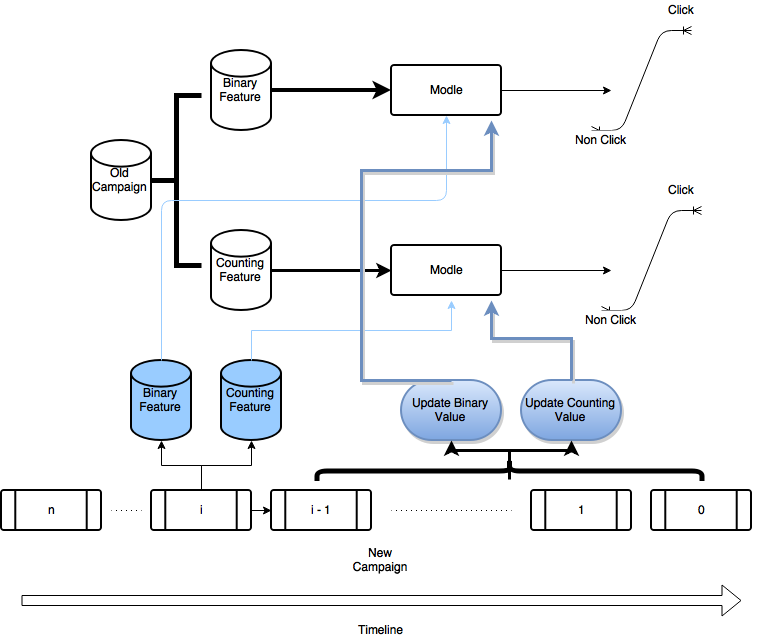
\includegraphics[width=\columnwidth]{countingdiagram.png}
\caption{Estimate new campaign CTR using Binary Feature and Counting Feature Comparison}
\label{fig:binary}
\end{figure}




\subsection{Performance Comparison of Binary and Counting Feature in CTR prediction Problem}

In this section two experiments are conducted to compare the CTR prediction performance of Binary and Counting feature in terms of logistic regression and gradient boosting regression tree (GBRT) model. The first experiment is based on the public dataset from Ipinyou, which was released by the Chinese RTB company Ipinyou for global RTB algorithm competition in 2013. The dataset includes logs of ad auctions, bids, impressions, and also clicks \ref{zhang2014real}. All the features except for \textit{Usertag} are used in the experiment due to the bias in that feature. The result is as follows:





\begin{figure}[h]
\centering
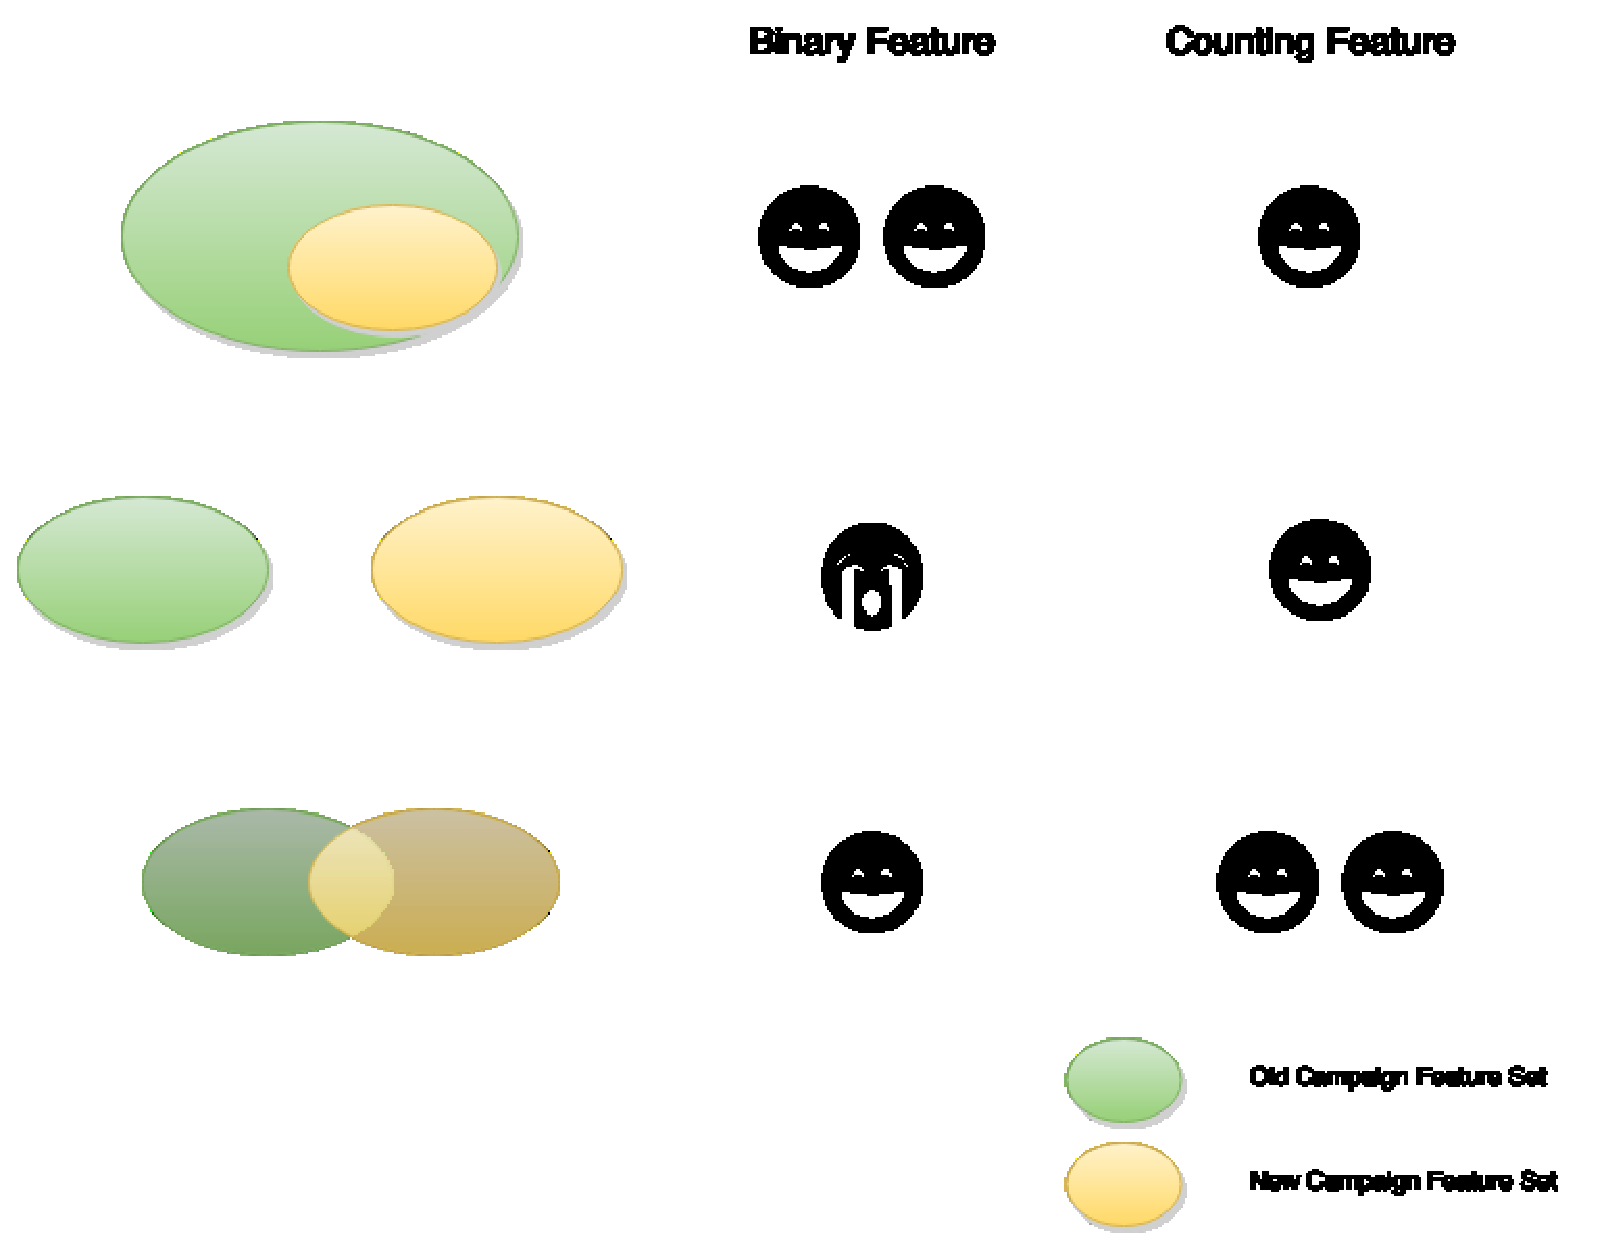
\includegraphics[width=\columnwidth]{Datasetbias.eps}
\caption{Three types of relation of feature sets between train dataset and test dataset}
\label{fig:datasetbias}
\end{figure}

\subsection{Performance Comparison of Binary and Counting Feature in Cold Start Problem}

In this part, the experiments will be done based on the dataset provided by a ad company in March which includes the data for 14 consecutive days, the dataset are separated by client id so that in each small dataset there are only the impressions from one unique client. In this experiment, the client with more than 500,000 impression are chosen so that 4 sub datasets are obtained which are from distinct clients. The detail of the four clients are shown in Table~\ref{tab:campainid}.


\begin{table}[t]
\centering
\begin{tabular}{c | c | c | c }
· 
\end{tabular}
\caption{Statistical Information of top 10 advertisement clients}
\label{tab:campainid}
\end{table}

\iffalse
\begin{table}[t]
 \centering
 \begin{tabular}{ ||c c || } 
 \hline
 Client id  & Number \\
 \hline
 20762 & 1068606 \\ 
  15140 & 764355 \\ 
   1371 & 576709 \\ 
   12482 & 557120\\
 \hline
 \end{tabular}
 \caption{Four Biggest clients}
 \label{tab:campainid}
 \end{table}
 
\fi

The figure above shows the truth that dataset significantly decide upper bound of the accuracy to predict CTR. above performance comparison of binary feature and counting feature on CTR estimation reveals that performance of counting feature using non-linear regression model is comparable to that of binary feature using linear regression model, the precondition is that the training and test dataset share most of the features. However, in real world we will always be faced up with the situation that the information is unbalanced in train and test dataset. We define \textit{Feature Set} as a criterion to measure the information obtained in the dataset, which is represented by  \(S_i(f)\), in which \(f\) are the unique features in the dataset \(i\).\vspace{5mm}

The relation of the feature sets in dataset \(i\) and \(j\) can be catogrized into three types, in which \(i\) is the test dataset, and \(j\) is the training dataset, as shown in Figure~\ref{fig:datasetbias}.:
\begin{itemize}
\item When \(s_i \subset s_j\), the binary feature should perform better than counting feature in terms of CTR estimation. Since in this way all the feature information needed by test dataset is inclusive in training dataset, the model contains all the infomraiton as a general model, as with the above conclusion when both using linear logistic regression, binary feature is superior to counting feature.  
\item When \(s_i \cap s_j \equiv 0\), the counting feature should perform better than binary feature which degenerates into random algorithm. The reason is that there is no overlap between \(s_i\) and \(s_j)\), so all feature information in test dataset will be regared as \textit{other} for model derived from training dataset. However, for counting feature, this deficiency can be made up with the gradual increasing information of the dataset distribution. The counting value to some extent represents the feature distribution so when we assume that the train and test dataset share similar feature value distribution counting feature can still perform rather well while at same time prediction using binary feature is totoally impossible.
\item When \(s_i \cap s_j \neq 0\), the feature informaiton at this time is shared by train and test dataset. We define \textit{General Information} as the information shared by all the advertisement campaigns, and \textit{Specific Information} as the unique feature information owned by each of the campaign. In this situation, both binary feature and counting feature performs well granted that train and test dataset share enough feature information so that the model to some extent is universal among datasets. However, the upper-bound of performance of binary feature is around the AUC result of the CTR prediction for first data capsule in the data stream assuming the distribution among test dataset is identical, conversely, that is the lower-bound of the performance of counting feature since with the increasing of test instances, counting value will tend towards the real distribution of test dataset to compensate of the unbalanced counting weights value. 
\end{itemize}



\begin{figure}[t]
\centering
\includegraphics[width=\columnwidth]{coldstart_first.eps}
\caption{Performance Comparison of Binary and Counting feature for Cross Domain Learning before Counting Value Updating}
\label{fig:coldstart_first}
\end{figure}

\begin{figure}[t]
\centering
\includegraphics[width=\columnwidth]{coldstart.eps}
\caption{Performance Comparison of Binary and Counting feature for Cross Domain Learning after convergence}
\label{fig:coldstart}
\end{figure}

\begin{figure}[t]
\centering
\includegraphics[width=\columnwidth]{coldstartimprove.eps}
\caption{Performance Comparison of Binary and Counting feature for Cross Domain Learning after convergence}
\label{fig:coldstartimprove}
\end{figure}

Figure \ref{fig:coldstart_first} shows the comparison of the performance between binary feature and counting feature before updating counting values. As shown in the diagram above, for binary feature the counting value will be updated between 0 and 1 since it is discrete, however, because the values of counting feature is continuous, so it is possible to update its values with the introduction of new data from new campaign. Figure \ref{fig:coldstart_first} shows the fact that just after training the model from old campaign, directly using it to predict the CTR of new campaign, binary and counting features are suffering from the same bad performance. 

Figure \ref{fig:coldstart} shows the fact that counting feature indeed improve the performance of CTR prediction after a few times updating until convergence. After getting information from the new coming data, the counting value will be changed to represent the distribution of the new campaign somehow, which takes over the responsibility from the binary weights space. However for binary feature since its feature space is fixed so changing between 0 and 1 cannot represent the distribution of the new campaign so there is no performance improvement for binary feature after the updating. 

Figure \ref{fig:coldstartimprove} demonstrates the conclusion in last above well. If we assume that the distribution of the new campaign is identical, the performance of the CTR prediction in terms of AUC should be the same among all sub-dataset of the new campaign. We define  \(AUC_{\text{before}}\) as the CTR prediction performance for the first capsule of new campaign data, when there is no counting value update from new campaign and we can only predict it based on the model from the old campaign. We also define \(AUC_{\text{after}}\) as the peformance of binary or counting feature after all the information of the new campaign has been obtained by the model and it becomes converged. In Figure \ref{fig:coldstartimprove} we compare the\({AUC_{\text{after}}}/{AUC_{\text{before}}}\)
for binary feature and counting feature.From the plot it shows that for binary feature there is no improvement for most cases since the value is around 1 and for counting feature the improvement is high. 



Figure \ref{fig:matrixbefore} \ref{fig:matrixafter} and \ref{fig:matriximprove} shows the details of the result.In Figure \ref{fig:matrixbefore} we calculate \((AUC_{\text{before(count)}} - AUC_{\text{before(bi)}}) / AUC_{\text{before(bi)}} \) to show how counting feature improves the performance compared to binary feature before updating the counting values, the result shows that counting feature performs bad which is not surprising. 

In Figure \ref{fig:matrixafter} we shows the same calculating for that but after updating the counting values.  \((AUC_{\text{after(count)}} - AUC_{\text{after(bi)}}) / AUC_{\text{after(bi)}} \) is shown in the matrix. Green shows that the counting feature performs better than binary feature, and the percentage value shows by how many percents do the counting feature obtains in terms of CTR AUC performance. It shows that excluding the diagonal in which the train and test dataset are the same, so the binary feature should perform better than counting feature, In 61 out of 90 experiments counting feature performs better than binary feature, which is much better than we can see in Matrix \ref{fig:matrixbefore}.

Figure \ref{fig:matriximprove} calculates 
\((AUC_{\text{after(count)}}/AUC_{\text{before(count)}} -AUC_{\text{after(bi)}}/AUC_{\text{before(bi)}})  / (AUC_{\text{after(bi)}}/AUC_{\text{before(bi)}})  \), which shows that after updating the counting value, whether counting feature gains more performance improvement than binary feature, result shows that counting feature indeed improves much more than binary feature whose upper bound of CTR estimation is decided when the first subset of data comes. 

\begin{figure}[t]
\centering
\includegraphics[width=\columnwidth]{matrixbefore.eps}
\caption{Percentage of Performance Improvement of Counting Feature to Binary Feature in Cross Domain Learning before Counting Value Updating}
\label{fig:matrixbefore}
\end{figure}

\begin{figure}[t]
\centering
\includegraphics[width=\columnwidth]{matrixafter.eps}
\caption{Percentage of Performance Improvement of Counting Feature to Binary Feature in Cross Domain Learning After Convergence}
\label{fig:matrixafter}
\end{figure}

\begin{figure}[t]
\centering
\includegraphics[width=\columnwidth]{matriximprove.eps}
\caption{Percentage of Performance Improvement of Counting Feature Compared to Binary Feature}
\label{fig:matriximprove}
\end{figure}


\begin{figure}[t]
\centering
\includegraphics[width=\columnwidth]{variance.eps}
\caption{Cross-validation of binary and counting feature dataset mean and variance}
\label{fig:variance}
\end{figure}

\begin{figure}[t]
\centering
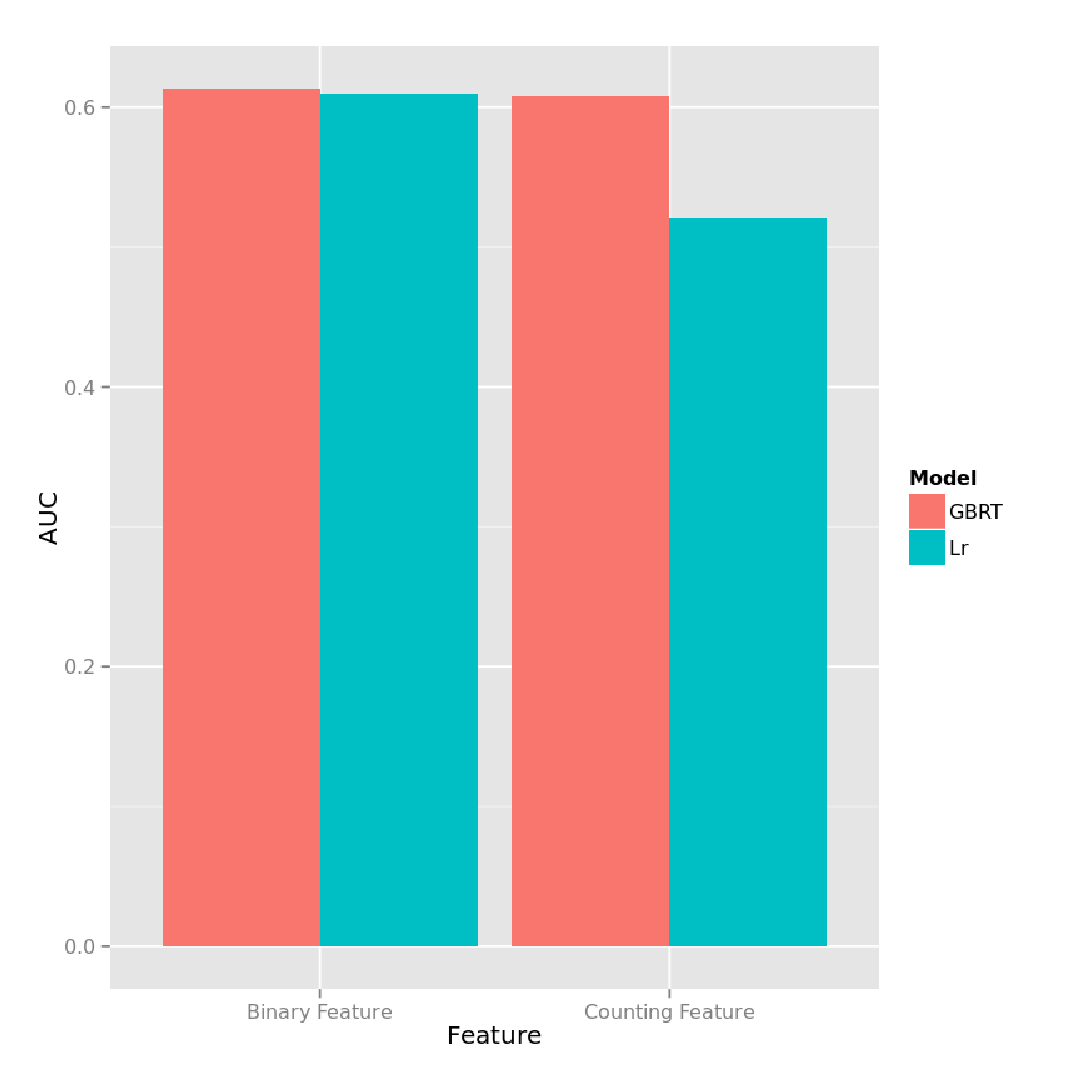
\includegraphics[width=\columnwidth]{2261.eps}
\caption{Performance 2261}
\label{fig:2261}
\end{figure}

\begin{figure}[t]
\centering
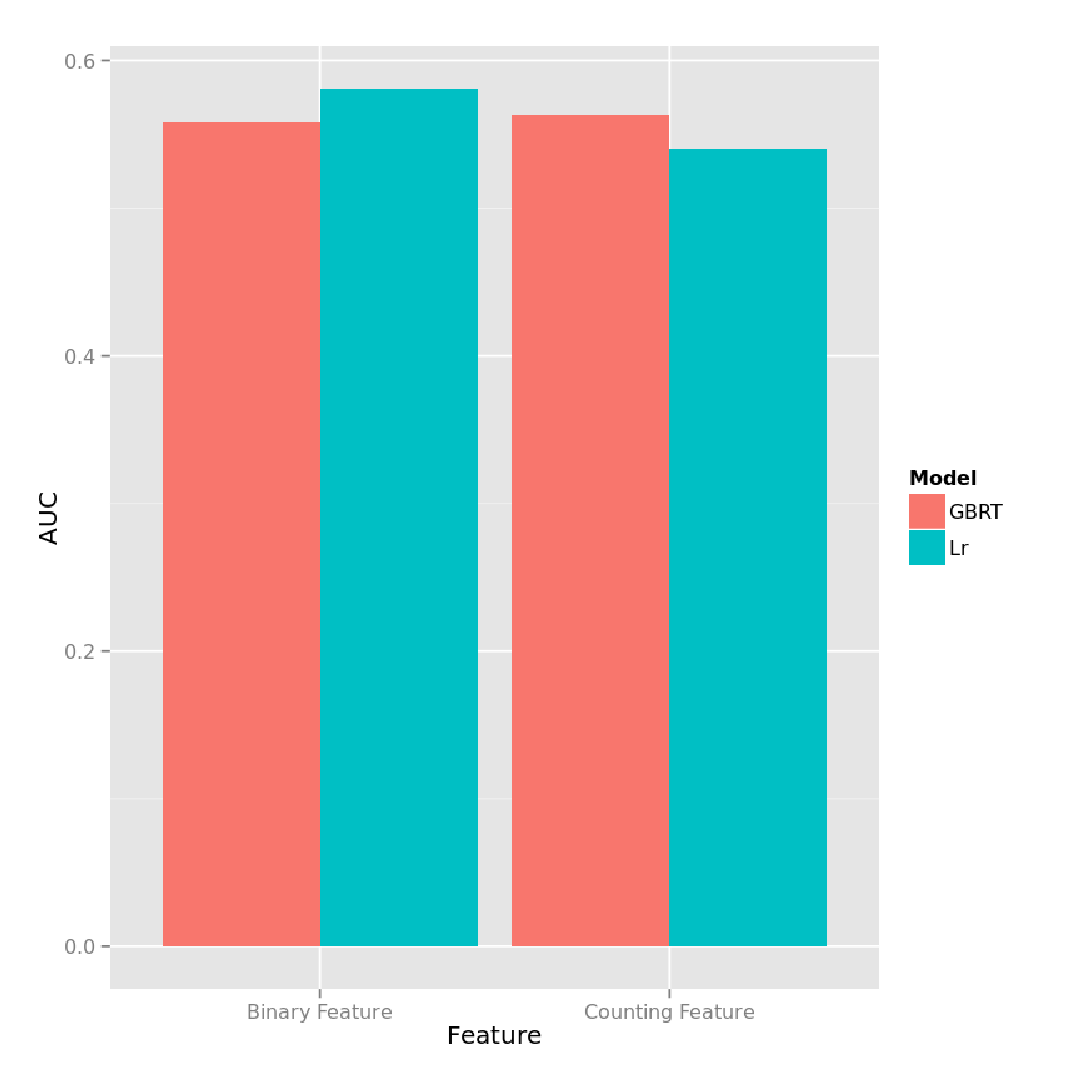
\includegraphics[width=\columnwidth]{2997.eps}
\caption{Performance 2997}
\label{fig:2997}
\end{figure}

\begin{figure}[t]
\centering
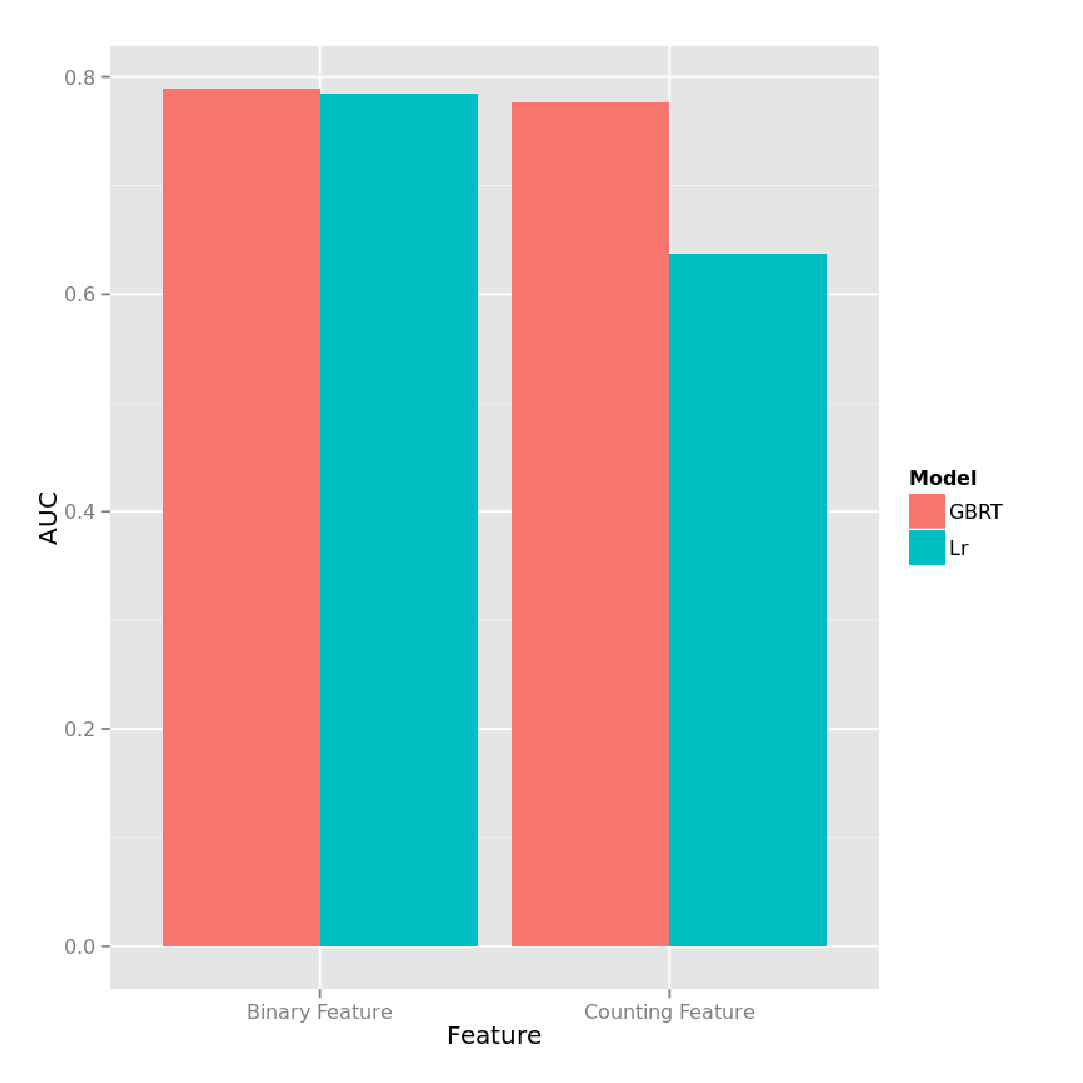
\includegraphics[width=\columnwidth]{3386.eps}
\caption{Performance 3386}
\label{fig:3386}
\end{figure}


% The data from 3-14 to 3-27 are regarded as training dataset, the data from 5- are regarded as test dataset, the count of training dataset is, test dataset is ~\ref{tab:campainid}

% \begin{table*}[h]
% \centering
% \begin{tabular}{ |c|c|c|c| } 
% \hline
% Shared Campaign  & Unique Train Dataset Campaign & Unique Test Dataset Campaign \\
% \hline
% 1310190 & 1307617, 884194, 1283235, 1335301  & 1466432, 1448738 \\ 
% & 1385319, 1349577, 1276074, 1363723 & 1406405, 1424966 \\ 
% &  1357245, 1341802, 1341937, 1307838 & 1424330, 1445998 \\ 
% &  1285558, 1358167, 1305663, 1299899 & 1458704, 1454382 \\
% &  1363711, 1386205, 1368830, 1366271 &  1472727, 1452138 \\
% \hline
% \end{tabular}
% \label{tab:campainid}
% \end{table}

% Only the instances from the campaign with more than 500 clicks and 50000 impressions will be remained, the campaigns can be classified as the ones shared by the training and test dataset, the ones unique to training dataset and the one unique to test dataset.  

% \(1/3\) of the training dataset is used as train dataset, \(2/3\) will be used as count dataset. In order to increase the generalization of training dataset to improve the universality of the trained prediction model, four campaign will constitute one training dataset and two campaigns are used to make up a test dataset to decrease the bias of test dataset.  

% For the sake of convenience, the training dataset will be labeled as 1,2,3,4 and 5, from top to the bottom, as well as the test dataset. For each training dataset, the prediction model will be build based on it which will be used to test the data stream from each of the test dataset, the result is in 6.3.


\begin{figure*}
    \centering
    \begin{subfigure}[b]{0.3\textwidth}
        \centering
        \includegraphics[width=\textwidth]{cos}
        \caption{Cos Similarity Comparison Between Pairwise of Binary Feature and Counting Feature}
        \label{fig:cos}
    \end{subfigure}
    \hfill
    \begin{subfigure}[b]{0.3\textwidth}
        \centering
        \includegraphics[width=\textwidth]{correlation}
        \caption{Correlation Similarity Comparison Between Pairwise of Binary Feature and Counting Feature}
        \label{fig:correlation}
    \end{subfigure}
    \hfill
    \begin{subfigure}[b]{0.3\textwidth}
        \centering
        \includegraphics[width=\textwidth]{euclidean}
        \caption{Euclidean Distance Comparison Between Pairwise of Binary Feature and Counting Feature}
        \label{fig:euclidean}
    \end{subfigure}
    \caption{Comparison of Binary and Counting Feature Model Weights Space}
    \label{fig:three graphs}
\end{figure*}


Figure \ref{fig:variance} shows that the variance and mean for binary and counting feature dataset are nearly the same. 

Figure \ref{fig:three graphs} shows that the similarity among weights space for counting feature is higher than counting feature. 



\iffalse
Experiment 1.1: Training Dataset  (20762), Test Dataset  (15140) in Figure~\ref{fig:fig1}.:
\begin{figure}[h]
\centering
\includegraphics[width=\columnwidth]{20762_15140.eps}
\caption{Training Dataset  (20762), Test Dataset  (15140)}
\label{fig:fig1}
\end{figure}

Experiment 1.2: Training Dataset  (20762), Test Dataset  (1371) in Figure~\ref{fig:fig2}.:
\begin{figure}[h]
\centering
\includegraphics[width=\columnwidth]{20762_1371.eps}
\caption{Training Dataset  (20762), Test Dataset  (1371)}
\label{fig:fig2}
\end{figure}

Experiment 1.3: Training Dataset  (20762), Test Dataset  (12482) in Figure~\ref{fig:fig2}.:
\begin{figure}[h]
\centering
\includegraphics[width=\columnwidth]{20762_12482.eps}
\caption{ Training Dataset  (20762), Test Dataset  (12482)}
\label{fig:fig2}
\end{figure}

Experiment 2.1: Training Dataset  (15140), Test Dataset  (20762) in Figure~\ref{fig:fig3}.:
\begin{figure}[h]
\centering
\includegraphics[width=\columnwidth]{15140_20762.eps}
\caption{Training Dataset  (15140), Test Dataset  (20762)}
\label{fig:fig3}
\end{figure}

Experiment 2.2: Training Dataset  (15140), Test Dataset  (1371) in Figure~\ref{fig:fig4}.:
\begin{figure}[h]
\centering
\includegraphics[width=\columnwidth]{15140_1371.eps}
\caption{Training Dataset  (15140), Test Dataset  (1371)}
\label{fig:fig4}
\end{figure}

Experiment 2.3: Training Dataset  (15140), Test Dataset  (12482) in Figure~\ref{fig:fig5}.:
\begin{figure}[h]
\centering
\includegraphics[width=\columnwidth]{15140_12482.eps}
\caption{Training Dataset  (15140), Test Dataset  (12482) }
\label{fig:fig5}
\end{figure}

Experiment 3.1: Training Dataset  (1371), Test Dataset  (20762) in Figure~\ref{fig:fig6}.:
\begin{figure}[h]
\centering
\includegraphics[width=\columnwidth]{1371_20762.eps}
\caption{ Training Dataset  (1371), Test Dataset  (20762)}
\label{fig:fig6}
\end{figure}

Experiment 3.2: Training Dataset  (1371), Test Dataset  (15140) in Figure~\ref{fig:fig7}.:
\begin{figure}[h]
\centering
\includegraphics[width=\columnwidth]{1371_15140.eps}
\caption{Training Dataset  (1371), Test Dataset  (15140)}
\label{fig:fig7}
\end{figure}

Experiment 3.3: Training Dataset  (1371), Test Dataset  (12482) in Figure~\ref{fig:fig8}.:
\begin{figure}[h]
\centering
\includegraphics[width=\columnwidth]{1371_12482.eps}
\caption{Training Dataset  (1371), Test Dataset  (12482)}
\label{fig:fig8}
\end{figure}

Experiment 4.1: Training Dataset  (12482), Test Dataset  (20762) in Figure~\ref{fig:fig9}.:
\begin{figure}[h]
\centering
\includegraphics[width=\columnwidth]{12482_20762.eps}
\caption{Training Dataset  (12482), Test Dataset  (20762)}
\label{fig:fig9}
\end{figure}

Experiment 4.2: Training Dataset  (12482), Test Dataset  (1371) in Figure~\ref{fig:fig10}.:
\begin{figure}[h]
\centering
\includegraphics[width=\columnwidth]{12482_1371.eps}
\caption{Training Dataset  (12482), Test Dataset  (1371)}
\label{fig:fig10}
\end{figure}

Experiment 4.2: Training Dataset  (12482), Test Dataset  (15140) in Figure~\ref{fig:fig11}.:
\begin{figure}[h]
\centering
\includegraphics[width=\columnwidth]{12482_15140.eps}
\caption{Training Dataset  (12482), Test Dataset  (15140)}
\label{fig:fig11}
\end{figure}

\fi



\chapter{Conclusions and Future Work}
\label{conclusion}
In this project, we introduce the concept of \textit{counting feature} which is composed of \textit{frequency feature} and \textit{average CTR feature}, and prove that for the same dataset, counting feature space is a non-linear transformation of binary feature space, and the CTR prediction performance in terms of AUC of counting feature using GBRT algorithm is comparable to that of binary feature using linear logistic regression model. Unlike previous and current researches which focus more on the improvement of machine learning model and algorithm in CTR prediction problem, we turn to the more fundamental, but more crucial to the industry, research field, which is feature engineering. We show that counting feature can not only transform the extremely high dimension feature space into low, scalable, interpretable space, but also remain the comparable CTR prediction performance as traditional method, which will largely decrease the memory and time cost for industry. 

To the best of our knowledge, our work is the first one to systematically research on statistical feature, namely counting feature, even though statistical feature has been used by a small range of companies in daily business, our work is the first one to not only provide experimental result, but also mathematical derivation. The most important thing is, we present that counting feature can partly solve the classical \textit{cold start} problem to extend the knowledge from one advertising campaign to the others, we show that without updating old model parameters we can still obtain high performance using counting feature in the context of \textit{cross-domain learning} problem. There are few literature studying on cross-domain learning problem in the field of online advertising, and we are the first one with simplest implementation and solid backups.

However, the research in of our work is not ended. Firstly, we need more dataset to test our theory since currently we only have two datasets which are from iPinYou and Adform, also more linear and non-linear machine learning algorithms should be used to validate the correctness of our theory. Secondly, now we can only do the offline experiment, however, since for cross-learning problem, commonly the new income data should be in the format of stream, we already mimic the process of data stream, but implementing the experiment online will be absolutely what we will do next. Lastly, for the cross-learning problem, now we assume that the marginal distribution of the joint probability distribution of feature and label space are the same so that directly using model from old campaign to new ones is feasible, however, the covariate or domain shift is inevitable in the real world machine learning problem, a multitask optimization method to not only minimise the different between the feature distribution of source and target campaign, but also classifier difference should be studied to increase the CTR prediction further.

%\addcontentsline{toc}{chapter}{Appendices}

% The \appendix command resets the chapter counter, and changes the chapter numbering scheme to capital letters.
%\chapter{Appendices}
\appendix
\chapter{List of Code}
\label{appendixlabel1}
1. Make Feature \\
(1). Make Binary Feature
\lstset{language=Python, 
        basicstyle=\ttfamily\small, 
        keywordstyle=\color{blue},
        commentstyle=\color{comments},
        stringstyle=\color{black},
        showstringspaces=false,
        identifierstyle=\color{black}}
\begin{lstlisting}[numbers=left, breaklines=true]
import pandas as pd
import sys
import numpy as np
import operator
import random
from collections import Counter
from math import sqrt
from random import shuffle
import math
def getsecondfeature(frame_train_count):
    columns1= ['log_date', 'log_time_hour', 'client_id', 'placement_id', \\
    'inventory_source_id', 'url', 'position_id', 'size', 'browser_id', \\
'os_id', 'user_agent', 'screen_size_id', 'visited_domains', 'visited_logpoints', 'clicker']
    count_valid = {}
    second = {}
    second_valid = {}
    second_whole = []

    for idx1, val1 in enumerate(columns1):
        for idx2, val2 in enumerate(columns1[idx1+1:]):
            second[val1] = frame_train_count.groupby([val1, val2])\\
            [val1].count()
            second_valid[val1] = [key for key in second[val1].keys() if \\
            second[val1][key] > 10000]
            second_whole.extend(second_valid[val1])
            second_whole.append(val1+':other')\\
    return second_whole

def notlast(itr):
    itr = iter(itr)  # ensure we have an iterator
    prev = itr.next()
    for item in itr:
        yield prev

        prev = item
print 'start'
file = sys.argv[1]
file = int(float(file))
cnt = Counter()
ctrcount = Counter()
pd.options.display.float_format = '{:.25f}'.format

columns = ['log_date', 'log_time_hour',
           'inventory_source_id', 'position_id', 'size', 'browser_id', 'os_id', 'user_agent',
           'screen_size_id', 'visited_domains', 'visited_logpoints', 'clicker', 'click_count']

columns1= ['log_date', 'log_time_hour', 'client_id', 'placement_id',
           'inventory_source_id', 'domain', 'url', 'position_id', 'size', 'browser_id', 'os_id', 'user_agent',
           'screen_size_id', 'visited_domains', 'visited_logpoints', 'clicker']

path_train_train = '%d/train.train.txt' % file
path_train_count = '%d/train.count.txt' %file
path_test_test = '%d/test.test.txt' % file
path_test_valid = '%d/test.valid.txt' % file

fo_train = open('%d/train.bi.txt' %file, 'w')
fo_test_test = open('%d/test.bi.test.txt' % file, 'w')
fo_test_valid = open('%d/test.bi.valid.txt' % file, 'w')
fo_index = open('%d/index.txt' % file, 'w')

frame_train_train = pd.read_csv(path_train_train,dtype=str,\\
error_bad_lines = False)
frame_train_count = pd.read_csv(path_train_count,dtype=str,\\
error_bad_lines = False)
frame_test_test = pd.read_csv(path_test_test,dtype=str,\\
error_bad_lines = False)
frame_test_valid = pd.read_csv(path_test_valid,dtype=str,\\
error_bad_lines = False)
total_length = len(frame_train_count)
dict_unique = {}

length = 0
frame_train_count = pd.DataFrame(frame_train_count, columns=columns)

for c_index in range(0, len(columns) - 1):
    seri_train_count = frame_train_count.ix[1:len(frame_train_count)-1,\\
    c_index]

    seri_train_count = seri_train_count[~seri_train_count.isnull()]
    unique_s = seri_train_count.unique()
    unique_s = unique_s.tolist() + ['other']
    index = 0
    unique_list = []
    dict_u = {}
    for u in range(0, len(unique_s)):
        dict_u[unique_s[u]] = u + length
    dict_unique[columns[c_index]] = dict_u
    length = length + len(unique_s)
index = 0
record_length = 0
for column in notlast(columns):
    index = index + 1
    dict_u = dict_unique[column]
    record_length = record_length + len(dict_u)
    for key in dict_u:
        fo_index.write(str(index) + ':' + str(key) + ' ' + str(dict_u[key]))
        fo_index.write('\n')
record_length = record_length + 100
record_length = 2155314

        # ctr[column] = (frame_train_ctr.groupby(column).size()/float(count[column])).fillna(0)
for index, row in frame_train_train.iterrows():
    if row[-1] == str(0) or row[-1] == 0:
        fo_train.write(str(0))
    else:
        fo_train.write(str(1))

    for column in notlast(columns):
        dict_u = dict_unique[column]
        if row[column] not in dict_u:
            id = dict_u['other']
            fo_train.write(' ' + str(id) + ':' + str(1))
        else:
            id = dict_u[row[column]]
            fo_train.write(' ' + str(id) + ':' + str(1))

    fo_train.write('\n')
fo_train.close()

for index, row in frame_test_test.iterrows():
    if row[-1] == str(0) or row[-1] == 0:
        fo_test_test.write(str(0))
    else:
        fo_test_test.write(str(1))

    for column in notlast(columns):
        dict_u = dict_unique[column]
        if row[column] not in dict_u:
            id = dict_u['other']
            fo_test_test.write(' ' + str(id) + ':' + str(1))
        else:
            id = dict_u[row[column]]
            fo_test_test.write(' ' + str(id) + ':' + str(1))

    fo_test_test.write('\n')
fo_test_test.close()

\end{lstlisting}
(2) Make Counting Feature
\lstset{language=Python, 
        basicstyle=\ttfamily\small, 
        keywordstyle=\color{blue},
        commentstyle=\color{comments},
        stringstyle=\color{black},
        showstringspaces=false,
        identifierstyle=\color{black}}
\begin{lstlisting}[numbers=left, breaklines=true]
import pandas as pd
import sys
import operator
import random
from collections import Counter
from math import sqrt
from random import shuffle
import math
import matplotlib.pyplot as plt
import numpy as np

def notlast(itr):
    itr = iter(itr)  # ensure we have an iterator
    prev = itr.next()
    for item in itr:
        yield prev
        prev = item
def median(mylist):
    sorts = sorted(mylist)
    length = len(sorts)
    if not length % 2:
        return (sorts[length / 2] + sorts[length / 2 - 1]) / 2.0
    return sorts[length / 2]

def k_means(data_pts, k=None):
    """ Helper functions """

    def lists_are_same(la, lb):  # see if two lists have the same elements
        out = False
        for item in la:
            if item not in lb:
                out = False
                break
            else:
                out = True
        return out

    def distance(a, b):  # distance between (x,y) points a and b
        return sqrt(abs(a[0] - b[0]) ** 2 + abs(a[1] - b[1]) ** 2)

    def average(a):  # return the average of a one-dimensional list (e.g., [1, 2, 3])
        return sum(a) / float(len(a))

    """ Set up some initial values """
    if k is None:  # if the user didn't supply a number of means to look for, try to estimate how many there are
        n = len(data_pts)  # number of points in the dataset
        k = int(sqrt(n / 2))  # number of clusters - see
        #   http://en.wikipedia.org/wiki/Determining_the_number_of_clusters_in_a_data_set#Rule_of_thumb
    if k < 1:  # make sure there's at least one cluster
        k = 1

    """ Randomly generate k clusters and determine the cluster centers,
        or directly generate k random points as cluster centers. """

    init_clusters = data_pts[:]  # put all of the data points into clusters
    shuffle(init_clusters)  # put the data points in random order
    init_clusters = init_clusters[0:k]  # only keep the first k random clusters

    old_clusters, new_clusters = {}, {}
    for item in init_clusters:
        old_clusters[item] = []  # every cluster has a list of points associated with it. Initially, it's 0

    while 1:  # just keep going forever, until our break condition is met
        tmp = {}
        for k in old_clusters:  # create an editable version of the old_clusters dictionary
            tmp[k] = []

        """ Associate each point with the closest cluster center. """
        for point in data_pts:  # for each (x,y) data point
            min_clust = None
            min_dist = 1000000000  # absurdly large, should be larger than the maximum distance for most data sets
            for pc in tmp:  # for every possible closest cluster
                pc_dist = distance(point, pc)
                if pc_dist < min_dist:  # if this cluster is the closest, have it be the closest (duh)
                    min_dist = pc_dist
                    min_clust = pc
            tmp[min_clust].append(point)  # add each point to its closest cluster's list of associated points

        """ Recompute the new cluster centers. """
        for k in tmp:
            associated = tmp[k]
            xs = [pt[0] for pt in associated]  # build up a list of x's
            ys = [pt[1] for pt in associated]  # build up a list of y's
            x = average(xs)  # x coordinate of new cluster
            y = average(ys)  # y coordinate of new cluster
            new_clusters[(
            x, y)] = associated  # these are the points the center was built off of, they're *probably* still associated

        if lists_are_same(old_clusters.keys(), new_clusters.keys()):  # if we've reached equilibrium, return the points
            return old_clusters.keys()
        else:  # otherwise, we'll go another round. let old_clusters = new_clusters, and clear new_clusters.
            old_clusters = new_clusters
            new_clusters = {}

file = sys.argv[1]
file = int(float(file))
cnt = Counter()
ctrcount = Counter()
count = {}
ctr = {}
test_count = {}
pd.options.display.float_format = '{:.25f}'.format

columns = ['log_date', 'log_time_hour',
           'inventory_source_id', 'position_id', 'size', 'browser_id', 'os_id', 'user_agent',
           'screen_size_id', 'visited_domains', 'visited_logpoints', 'clicker', 'click_count']

path_train_train = '%d/train.train.txt' % file
path_train_count = '%d/train.count.txt' % file
path_test_test = '%d/test.test.txt' % file
path_test_valid = '%d/test.valid.txt' % file

fo_train = open('%d/train.countfeature.txt' % file, 'w')
fo_test_test = open('%d/test.countfeature.test.txt' % file, 'w')
fo_test_valid = open('%d/test.countfeature.valid.txt' % file, 'w')
fo_index = open('%d/index_count.txt' % file, 'w')
fo_count_index = open('%d/index_countfeature.txt' % file, 'w')

index = 0
for column in notlast(columns):

    fo_count_index.write(column + ':' + 'frequency' + ' ' + str(index))
    index = index + 1
    fo_count_index.write('\n')
    fo_count_index.write(column + ':' + 'averagectr' + ' ' + str(index))
    index = index + 1
    fo_count_index.write('\n')

#print 'start'
frame_train_train = pd.read_csv(path_train_train, dtype=str,error_bad_lines = False)
frame_train_count = pd.read_csv(path_train_count, dtype=str,error_bad_lines = False)
frame_test_test = pd.read_csv(path_test_test, dtype=str,error_bad_lines = False)
frame_test_valid = pd.read_csv(path_test_valid, dtype=str,error_bad_lines = False)
total_length = len(frame_train_count)
test_total_length = len(frame_test_test)

for column in columns:
    count[column] = frame_train_count.groupby(column).size()
    test_count[column] = frame_test_test.groupby(column).size()

frame_train_ctr = frame_train_count[(frame_train_count.click_count == str(1))]
aver_count = {}
aver_ctr = {}

index = 1
for column in notlast(columns):
    count[column] = count[column].astype(float)
    #ctr[column] = math.log10((frame_train_ctr.groupby(column).size() / count[column]).fillna(0) + math.pow(10, -100))
    ctr[column] = ((frame_train_ctr.groupby(column).size() / count[column]).fillna(0))

    test_count[column] = test_count[column].astype(float)/float(test_total_length)
    count[column] = count[column].astype(float)/float(total_length)

    l = count[column].values.tolist()
    lctr = ctr[column].values.tolist()
    if len(l) == 0:
        aver_count[column] = 0

    else:
        aver_count[column] = sum(l)/float(len(l))
    if len(lctr) == 0:
        aver_ctr[column] = 0

    else:
        aver_ctr[column] = sum(lctr)/float(len(lctr))
        
# ctr[column] = (frame_train_ctr.groupby(column).size()/float(count[column])).fillna(0)
for index, row in frame_train_train.iterrows():
    id = 0
    if row[-1] == str(0) or row[-1] == 0:
        fo_train.write(str(0))
    else:
        fo_train.write(str(1))

    for column in notlast(columns):

        if column != 'click_count':

            if row[column] in count[column]:
                fo_train.write(' ' + str(id) + ':' + str(count[column][row[column]]))
                id = id + 1
                fo_train.write(' ' + str(id) + ':' + str(ctr[column][row[column]]))
                id = id + 1
            else:


                fo_train.write(' ' + str(id) + ':' + str(aver_count[column]))
                id = id + 1
                fo_train.write(' ' + str(id) + ':' + str(aver_ctr[column]))
                id = id + 1
    fo_train.write('\n')

fo_train.close()

for index, row in frame_test_test.iterrows():

    id = 0
    if row[-1] == str(0) or row[-1] == 0:
        fo_test_test.write(str(0))
    else:
        fo_test_test.write(str(1))

    for column in notlast(columns):

        if column != 'click_count':

            if row[column] in count[column]:

                fo_test_test.write(' ' + str(id) + ':' + str(count[column][row[column]]))
                id = id + 1
                fo_test_test.write(' ' + str(id) + ':' + str(ctr[column][row[column]]))
                id = id + 1
            else:
                fo_test_test.write(' ' + str(id) + ':' + str(aver_count[column]))
                id = id + 1
                fo_test_test.write(' ' + str(id) + ':' + str(aver_ctr[column]))
                id = id + 1
    fo_test_test.write('\n')

fo_test_test.close() 
\end{lstlisting}
2 Cold Start Experiment for Binary Feature
\lstset{language=Python, 
        basicstyle=\ttfamily\small, 
        keywordstyle=\color{blue},
        commentstyle=\color{comments},
        stringstyle=\color{black},
        showstringspaces=false,
        identifierstyle=\color{black}}
\begin{lstlisting}[numbers=left, breaklines=true]
import pandas as pd
import sys
import operator
import random
from collections import Counter
from math import sqrt
import math
import matplotlib.pyplot as plt
import collections
from random import shuffle
import subprocess
import os
import numpy as np


def log_10_product(x, pos):
    """The two args are the value and tick position.
    Label ticks with the product of the exponentiation"""
    return '%1i' % (x)


def k_means(data_pts, k=None):
    """ Helper functions """

    def lists_are_same(la, lb):  # see if two lists have the same elements
        out = False
        for item in la:
            if item not in lb:
                out = False
                break
            else:
                out = True
        return out

    def distance(a, b):  # distance between (x,y) points a and b
        return sqrt(abs(a[0] - b[0]) ** 2 + abs(a[1] - b[1]) ** 2)

    def average(a):  # return the average of a one-dimensional list (e.g., [1, 2, 3])
        return sum(a) / float(len(a))

    """ Set up some initial values """
    if k is None:  # if the user didn't supply a number of means to look for, try to estimate how many there are
        n = len(data_pts)  # number of points in the dataset
        k = int(sqrt(n / 2))  # number of clusters - see
        #   http://en.wikipedia.org/wiki/Determining_the_number_of_clusters_in_a_data_set#Rule_of_thumb
    if k < 1:  # make sure there's at least one cluster
        k = 1

    """ Randomly generate k clusters and determine the cluster centers,
        or directly generate k random points as cluster centers. """

    init_clusters = data_pts[:]  # put all of the data points into clusters
    shuffle(init_clusters)  # put the data points in random order
    init_clusters = init_clusters[0:k]  # only keep the first k random clusters

    old_clusters, new_clusters = {}, {}
    for item in init_clusters:
        old_clusters[item] = []  # every cluster has a list of points associated with it. Initially, it's 0

    while 1:  # just keep going forever, until our break condition is met
        tmp = {}
        for k in old_clusters:  # create an editable version of the old_clusters dictionary
            tmp[k] = []

        """ Associate each point with the closest cluster center. """
        for point in data_pts:  # for each (x,y) data point
            min_clust = None
            min_dist = 1000000000  # absurdly large, should be larger than the maximum distance for most data sets
            for pc in tmp:  # for every possible closest cluster
                pc_dist = distance(point, pc)
                if pc_dist < min_dist:  # if this cluster is the closest, have it be the closest (duh)
                    min_dist = pc_dist
                    min_clust = pc
            tmp[min_clust].append(point)  # add each point to its closest cluster's list of associated points

        """ Recompute the new cluster centers. """
        for k in tmp:
            associated = tmp[k]
            xs = [pt[0] for pt in associated]  # build up a list of x's
            ys = [pt[1] for pt in associated]  # build up a list of y's
            x = average(xs)  # x coordinate of new cluster
            y = average(ys)  # y coordinate of new cluster
            new_clusters[(
                x,
                y)] = associated  # these are the points the center was built off of, they're *probably* still associated

        if lists_are_same(old_clusters.keys(), new_clusters.keys()):  # if we've reached equilibrium, return the points
            return old_clusters.keys()
        else:  # otherwise, we'll go another round. let old_clusters = new_clusters, and clear new_clusters.
            old_clusters = new_clusters
            new_clusters = {}


def getplacement(path_train):
    frame_train = pd.read_csv(path_train)
    count = {}
    ctr = {}
    length = len(frame_train)
    frame_train_count = frame_train
    # print frame_train[:10]
    column = 'placement_id'

    count[column] = frame_train_count.groupby(column).size()
    count[column] = count[column].astype(float)
    frame_train_ctr = frame_train_count[(frame_train_count.click_count == 1)]
    ctr[column] = frame_train_ctr.groupby(column).size()
    dict_count = count[column]
    dict_ctr = ctr[column]
    clickhuge = [k for k in dict_ctr.keys() if dict_ctr[k] >= 500 and dict_count[k] >= 30000]

    return (count, ctr, clickhuge)

def getclient(path_train):
    frame_train = pd.read_csv(path_train)
    count = {}
    ctr = {}
    length = len(frame_train)
    frame_train_count = frame_train
    # print frame_train[:10]
    column = 'client_id'

    count[column] = frame_train_count.groupby(column).size()
    count[column] = count[column].astype(float)
    frame_train_ctr = frame_train_count[(frame_train_count.click_count == 1)]
    ctr[column] = frame_train_ctr.groupby(column).size()
    dict_count = count[column]
    dict_ctr = ctr[column]
    clickhuge = [k for k in dict_ctr.keys() if dict_ctr[k] >= 400]
    return (count, ctr, clickhuge)


cnt = Counter()
ctrcount = Counter()
pd.options.display.float_format = '{:.30f}'.format
file = sys.argv[1]
file = int(float(file))

path_train = '%d/train.log.txt' % file
path_test = '%d/test.log.txt' % file

ccc1 = []
ccc2 = []

cc1 = []
cc2 = []
c1 = sys.argv[2]
c1 = int(float(c1))
cc1.append(c1)
c2 = sys.argv[3]
c2 = int(float(c2))
cc2.append(c2)
column = 'client_id'
frame_train = pd.read_csv(path_train)
frame_test = frame_train

ccc1 = cc1
frame_train_wihout_cc = frame_train.loc[frame_train[column].isin(ccc1)]
rows = random.sample(frame_train_wihout_cc.index, (len(frame_train_wihout_cc.index) / 3))
frame_train_train = frame_train_wihout_cc.ix[rows]
frame_train_count = frame_train_wihout_cc.drop(rows)
print 'step1'
#ccc2.append(cc2[1])
ccc2 = cc2
frame_test_with_cc = frame_train.loc[frame_train[column].isin(ccc2)]
frame_test_with_cc=frame_test_with_cc.iloc[np.random.permutation(len(frame_test_with_cc))]
frame_test_with_cc = frame_test_with_cc.reset_index(drop=True)

wholelength = len(frame_test_with_cc)
print wholelength
windowrange = 50000

frame_test_test = pd.DataFrame()
frame_test_test_update = pd.DataFrame()
pace = 0

fo_result = open('%d/performance_ten_bi_%d_%d.txt' % (file,c1,c2), 'w')
print len(frame_test_with_cc)
    
print len(frame_train_train)
result = []
while (pace < wholelength - windowrange):
    new_data = frame_test_with_cc[pace:pace + windowrange - 1]
    
    if pace == 0:
        frame_train_train = [frame_train_train,frame_test_test[:windowrange/3]]
        frame_train_train = pd.concat(frame_train_train)
        frame_train_count = [frame_train_count,frame_test_test[(windowrange/3)+1:]]
        frame_train_count = pd.concat(frame_train_count)
        frame_test_test = new_data
        fo_train_train = open('%d/train.train.txt' % file, 'w')
        fo_train_count = open('%d/train.count.txt' % file, 'w')
        fo_test = open('%d/test.test.txt' % file, 'w')
        fo_test1 = open('%d/test.valid.txt' % file, 'w')

        frame_train_train.to_csv(fo_train_train, index=False)
        frame_train_count.to_csv(fo_train_count, index=False)
        frame_test_test.to_csv(fo_test, index=False)
        frame_test_test.to_csv(fo_test1, index=False)
        print pace/10000
        os.system("python -W ignore make_bi_new.py 11")
        rc = subprocess.Popen(['bash','/home/gaoxinyang/data/ctr-counting-features/models/lr/lr-driver.sh'],stdout=subprocess.PIPE)
        out = rc.communicate()[0]
        fo_result.write(out)
        fo_result.write('end')
    else:
    
        frame_test_test = new_data        
        #fo_train_count = open('%d/train.count.txt' % file, 'w')
        fo_test = open('%d/test.test.txt' % file, 'w')
        fo_test1 = open('%d/test.valid.txt' % file, 'w')

        frame_test_test.to_csv(fo_test, index=False)
        frame_test_test.to_csv(fo_test1, index=False)
        print pace/10000
        os.system("python -W ignore make_bi_new_update.py 11")
        #os.system("bash /home/gaoxinyang/data/ctr-counting-features/models/lr/lr-driver_update.sh")
        rc = subprocess.Popen(['bash','/home/gaoxinyang/data/ctr-counting-features/models/lr/lr-driver_update.sh'],stdout=subprocess.PIPE)
        out = rc.communicate()[0]
        fo_result.write(out)
        fo_result.write('end')
    pace = pace + windowrange
\end{lstlisting}
3. Cold Start for Counting Feature
\lstset{language=Python, 
        basicstyle=\ttfamily\small, 
        keywordstyle=\color{blue},
        commentstyle=\color{comments},
        stringstyle=\color{black},
        showstringspaces=false,
        identifierstyle=\color{black}}
\begin{lstlisting}[numbers=left, breaklines=true]
__author__ = 'gaoxinyang'
# !/usr/bin/python
__author__ = 'gaoxinyang'
import pandas as pd
import sys
import operator
import random
from collections import Counter
from math import sqrt
import math
import matplotlib.pyplot as plt
import collections
from random import shuffle
import subprocess
import os
import numpy as np


def log_10_product(x, pos):
    """The two args are the value and tick position.
    Label ticks with the product of the exponentiation"""
    return '%1i' % (x)


def k_means(data_pts, k=None):
    """ Helper functions """

    def lists_are_same(la, lb):  # see if two lists have the same elements
        out = False
        for item in la:
            if item not in lb:
                out = False
                break
            else:
                out = True
        return out

    def distance(a, b):  # distance between (x,y) points a and b
        return sqrt(abs(a[0] - b[0]) ** 2 + abs(a[1] - b[1]) ** 2)

    def average(a):  # return the average of a one-dimensional list (e.g., [1, 2, 3])
        return sum(a) / float(len(a))

    """ Set up some initial values """
    if k is None:  # if the user didn't supply a number of means to look for, try to estimate how many there are
        n = len(data_pts)  # number of points in the dataset
        k = int(sqrt(n / 2))  # number of clusters - see
        #   http://en.wikipedia.org/wiki/Determining_the_number_of_clusters_in_a_data_set#Rule_of_thumb
    if k < 1:  # make sure there's at least one cluster
        k = 1

    """ Randomly generate k clusters and determine the cluster centers,
        or directly generate k random points as cluster centers. """

    init_clusters = data_pts[:]  # put all of the data points into clusters
    shuffle(init_clusters)  # put the data points in random order
    init_clusters = init_clusters[0:k]  # only keep the first k random clusters

    old_clusters, new_clusters = {}, {}
    for item in init_clusters:
        old_clusters[item] = []  # every cluster has a list of points associated with it. Initially, it's 0

    while 1:  # just keep going forever, until our break condition is met
        tmp = {}
        for k in old_clusters:  # create an editable version of the old_clusters dictionary
            tmp[k] = []

        """ Associate each point with the closest cluster center. """
        for point in data_pts:  # for each (x,y) data point
            min_clust = None
            min_dist = 1000000000  # absurdly large, should be larger than the maximum distance for most data sets
            for pc in tmp:  # for every possible closest cluster
                pc_dist = distance(point, pc)
                if pc_dist < min_dist:  # if this cluster is the closest, have it be the closest (duh)
                    min_dist = pc_dist
                    min_clust = pc
            tmp[min_clust].append(point)  # add each point to its closest cluster's list of associated points

        """ Recompute the new cluster centers. """
        for k in tmp:
            associated = tmp[k]
            xs = [pt[0] for pt in associated]  # build up a list of x's
            ys = [pt[1] for pt in associated]  # build up a list of y's
            x = average(xs)  # x coordinate of new cluster
            y = average(ys)  # y coordinate of new cluster
            new_clusters[(
                x,
                y)] = associated  # these are the points the center was built off of, they're *probably* still associated

        if lists_are_same(old_clusters.keys(), new_clusters.keys()):  # if we've reached equilibrium, return the points
            return old_clusters.keys()
        else:  # otherwise, we'll go another round. let old_clusters = new_clusters, and clear new_clusters.
            old_clusters = new_clusters
            new_clusters = {}


def getplacement(path_train):
    frame_train = pd.read_csv(path_train)
    count = {}
    ctr = {}
    length = len(frame_train)
    frame_train_count = frame_train
    # print frame_train[:10]
    column = 'placement_id'

    count[column] = frame_train_count.groupby(column).size()
    count[column] = count[column].astype(float)
    frame_train_ctr = frame_train_count[(frame_train_count.click_count == 1)]
    ctr[column] = frame_train_ctr.groupby(column).size()
    dict_count = count[column]
    dict_ctr = ctr[column]
    clickhuge = [k for k in dict_ctr.keys() if dict_ctr[k] >= 500 and dict_count[k] >= 30000]

    return (count, ctr, clickhuge)

def getclient(path_train):
    frame_train = pd.read_csv(path_train)
    count = {}
    ctr = {}
    length = len(frame_train)
    frame_train_count = frame_train
    # print frame_train[:10]
    column = 'client_id'

    count[column] = frame_train_count.groupby(column).size()
    count[column] = count[column].astype(float)
    frame_train_ctr = frame_train_count[(frame_train_count.click_count == 1)]
    ctr[column] = frame_train_ctr.groupby(column).size()
    dict_count = count[column]
    dict_ctr = ctr[column]
    clickhuge = [k for k in dict_ctr.keys() if dict_ctr[k] >= 400]
    return (count, ctr, clickhuge)
cnt = Counter()
ctrcount = Counter()
pd.options.display.float_format = '{:.30f}'.format
file = sys.argv[1]
file = int(float(file))

path_train = '%d/train.log.txt' % file
path_test = '%d/test.log.txt' % file

# count_train, ctr_train, clickhuge_train = getplacement(path_train)

ccc1 = []
ccc2 = []
cc1 = []
c1 = sys.argv[2]
c1 = int(float(c1))
cc1.append(c1)

c2 = sys.argv[3]
c2 = int(float(c2))
cc2.append(c2)

ccc1 = cc1
frame_train_wihout_cc = frame_train.loc[frame_train[column].isin(ccc1)]
rows = random.sample(frame_train_wihout_cc.index, (len(frame_train_wihout_cc.index) / 3))
frame_train_train = frame_train_wihout_cc.ix[rows]
frame_train_count = frame_train_wihout_cc.drop(rows)
#ccc2.append(cc2[1])
ccc2 = cc2
frame_test_with_cc = frame_train.loc[frame_train[column].isin(ccc2)]
frame_test_with_cc=frame_test_with_cc.iloc[np.random.permutation(len(frame_test_with_cc))]
frame_test_with_cc = frame_test_with_cc.reset_index(drop=True)
#frame_test_with_cc = frame_test_with_cc.reindex(np.random.permutation(frame_test_with_cc.index))

wholelength = len(frame_test_with_cc)
#print wholelength
windowrange = 50000                          

frame_test_test = pd.DataFrame()
frame_test_test_update = pd.DataFrame()
pace = 0
fo_result = open('%d/performance_ten_count_%d_%d.txt' % (file,c1,c2), 'w')
result = []
while (pace < wholelength - windowrange):
    # if frame_test_with_cc.shape[0] > 150000: # len(df) > 10 would also work
    new_data = frame_test_with_cc[pace:pace + windowrange - 1]
    if pace == 0:
        frame_train_train = [frame_train_train,frame_test_test[:windowrange/3]]
        frame_train_train = pd.concat(frame_train_train)
        frame_train_count = [frame_train_count,frame_test_test[(windowrange/3)+1:]]
        frame_train_count = pd.concat(frame_train_count)

        frame_test_test = new_data
        fo_train_train = open('%d/train.train.txt' % file, 'w')
        fo_train_count = open('%d/train.count.txt' % file, 'w')
        fo_test = open('%d/test.test.txt' % file, 'w')
        fo_test1 = open('%d/test.valid.txt' % file, 'w')

        frame_train_train.to_csv(fo_train_train, index=False)
        frame_train_count.to_csv(fo_train_count, index=False)
        frame_test_test.to_csv(fo_test, index=False)
        frame_test_test.to_csv(fo_test1, index=False)
        os.system("python -W ignore make_count_new.py 11")
        #os.system("bash /home/gaoxinyang/data/ctr-counting-features/models/lr/lr-driver_count.sh")
        rc = subprocess.Popen(['bash','/home/gaoxinyang/data/ctr-counting-features/models/lr/lr-driver_count.sh'],stdout=subprocess.PIPE)

        out = rc.communicate()[0]
        fo_result.write(out)
        fo_result.write('end')
    else:
        
        frame_test_test_update = [frame_test_test_update,frame_test_test]
        frame_test_test_update  = pd.concat(frame_test_test_update)
        frame_test_test = new_data
        fo_train_count = open('%d/train.count.txt' % file, 'w')
        fo_test = open('%d/test.test.txt' % file, 'w')
        fo_test1 = open('%d/test.valid.txt' % file, 'w')
        frame_test_test_update.to_csv(fo_train_count, index=False)
        frame_test_test.to_csv(fo_test, index=False)
        frame_test_test.to_csv(fo_test1, index=False)
        
        os.system("python -W ignore make_count_new_update.py 11")
        #os.system("bash /home/gaoxinyang/data/ctr-counting-features/models/lr/lr-driver_count_update.sh")
        rc = subprocess.Popen(['bash','/home/gaoxinyang/data/ctr-counting-features/models/lr/lr-driver_count_update.sh'],stdout=subprocess.PIPE)
        out = rc.communicate()[0]
        fo_result.write(out)
        fo_result.write('end')
    pace = pace + windowrange
\end{lstlisting}
4. Marginal Distribution Generalization for Counting Feature (Similar to that of Binary Feature, and also for the generalization of feature space
\lstset{language=Python, 
        basicstyle=\ttfamily\small, 
        keywordstyle=\color{blue},
        commentstyle=\color{comments},
        stringstyle=\color{black},
        showstringspaces=false,
        identifierstyle=\color{black}}
\begin{lstlisting}[numbers=left, breaklines=true]
import datetime
import pprint

import numpy as np
import pandas as pd
from pandas.io.data import DataReader
import pylab as plt
import sklearn
from sklearn.cross_validation import train_test_split, KFold
from sklearn.linear_model import LinearRegression, LogisticRegression
from sklearn.metrics import mean_squared_error
from sklearn.pipeline import Pipeline
from sklearn.preprocessing import PolynomialFeatures
from sklearn.datasets import load_svmlight_file
from scipy import sparse

import pandas
import random
import math
from sklearn.metrics import roc_auc_score
from sklearn.metrics import confusion_matrix
from matplotlib import pyplot
from math import log
from collections import Counter
from sklearn.metrics import matthews_corrcoef


def sigmoid(p):
    p = max(p,-200)
    
    return 1.0 / (1.0 + math.exp(-p))

def pred(x,w_0,w):
    p = w_0
    
    for (feat, val) in x:
        
        if feat < 25:
          
          p += w[feat] * val 
    p = sigmoid(p)

    return p

def one_data_y_x(line,one_value):
    
    s = line.strip().replace(':', ' ').split(' ')

    
    y = int(s[0])
    x = []
    for i in range(1, len(s), 2):
        #val = 1
        if not one_value:
            
            try:
              val = float(s[i+1])
              #val = sigmoid(float(s[i+1])*weights[int(s[i])])
            except:
              val = 0
        x.append((int(s[i]), val))
    return (y, x)

def logistic_regression(one_v,feature_n,fi_train,fi_test,weights):
    np.random.seed(10)
    one_value = one_v
    k = 3
    learning_rate = 0.005
    weight_decay = 1E-30
    train_rounds = 10
    buffer_num = 1000000
    feature_index = {}
    index_feature = {}
    max_feature_index = 0
    feature_num = feature_n

    init_weight = 0.1
    w = np.zeros(feature_num)
    w_0 = 0

# train
    best_auc = 0.
    overfitting = False
    for round in range(1, train_rounds+1):
        
        #fi = open(sys.argv[1], 'r')
        line_num = 0
        train_data = []
        
        fi = open(fi_train, 'r')
        line_num = 0
        train_data = []
        while True:
            line = fi.readline().strip()
            
            if len(line) > 0:
                line_num = (line_num + 1) % buffer_num
                s = line.strip('\0').replace(':', ' ').split(' ')
                try:
                  train_data.append(one_data_y_x(line,one_value))
                except:
                  pass
                    
            if line_num == 0 or len(line) == 0:
                for data in train_data:
                    y = data[0]
                    x = data[1]
                # train one data
                    p = pred(x,w_0,w)
                    d = y - p
                    w_0 = w_0 * (1 - weight_decay) + learning_rate * d
                    for (feat, val) in x:
                        if feat < 25:
                            w[feat] = w[feat] * (1 - weight_decay) + learning_rate * d * val
                train_data = []
            if len(line) == 0:
                break
        fi.close()
        y = []
        yp = []
        fi = open(fi_test, 'r')
        for line in fi:
            s = line.strip('\0').replace(':', ' ').split(' ')
            if len(s) == 49:
              data = one_data_y_x(line,one_v)
              clk = data[0]
              pclk = pred(data[1],w_0,w)
              y.append(clk)
              yp.append(pclk)
        fi.close()
        ypp = map(lambda x: 1 if x > 0.5 else 0, yp)
        result = confusion_matrix(y,ypp)
        auc = roc_auc_score(y, yp)
        rmse = math.sqrt((mean_squared_error(y, yp)))
    
    return rmse
def create_lagged_series(symbol, start_date, end_date, lags=5):
    """
    This creates a pandas DataFrame that stores the percentage returns of the 
    adjusted closing value of a stock obtained from Yahoo Finance, along with 
    a number of lagged returns from the prior trading days (lags defaults to 5 days).
    Trading volume, as well as the Direction from the previous day, are also included.
    """

    # Obtain stock information from Yahoo Finance
    ts = DataReader(symbol, "yahoo", start_date-datetime.timedelta(days=365), end_date)

    # Create the new lagged DataFrame
    tslag = pd.DataFrame(index=ts.index)
    tslag["Today"] = ts["Adj Close"]
    tslag["Volume"] = ts["Volume"]

    # Create the shifted lag series of prior trading period close values
    for i in xrange(0,lags):
        tslag["Lag%s" % str(i+1)] = ts["Adj Close"].shift(i+1)

    # Create the returns DataFrame
    tsret = pd.DataFrame(index=tslag.index)
    tsret["Volume"] = tslag["Volume"]
    tsret["Today"] = tslag["Today"].pct_change()*100.0

    # If any of the values of percentage returns equal zero, set them to
    # a small number (stops issues with QDA model in scikit-learn)
    for i,x in enumerate(tsret["Today"]):
        if (abs(x) < 0.0001):
            tsret["Today"][i] = 0.0001

    for i in xrange(0,lags):
        tsret["Lag%s" % str(i+1)] = tslag["Lag%s" % str(i+1)].pct_change()*100.0

    tsret["Direction"] = np.sign(tsret["Today"])
    tsret = tsret[tsret.index >= start_date]
    return tsret
def validation_set_poly(random_seeds, degrees, X, y):
    """
    Use the train_test_split method to create a
    training set and a validation set (50% in each)
    using "random_seeds" separate random samplings over
    linear regression models of varying flexibility
    """
    sample_dict = dict([("seed_%s" % i,[]) for i in range(1, random_seeds+1)])
    
    for i in range(1, random_seeds+1):
        for d in range(1, degrees+1):
            polynomial_features = PolynomialFeatures(
                degree=d, include_bias=False
            )
            linear_regression = LogisticRegression()
            model = Pipeline([
                ("polynomial_features", polynomial_features),
                ("linear_regression", linear_regression)
            ])
            X_train, X_test, y_train, y_test = train_test_split(
                X, y, test_size=0.5, random_state=i
            )
            model.fit(X_train, y_train)
            # Calculate the test MSE and append to the
            # dictionary of all test curves
            y_pred = model.predict(X_test)
            
            test_mse = mean_squared_error(y_test, y_pred)
            print test_mse
            sample_dict["seed_%s" % i].append(test_mse)
           
    sample_dict["avg"] = np.zeros(degrees)
    for i in range(1, random_seeds+1):
        sample_dict["avg"] += sample_dict["seed_%s" % i]
    sample_dict["avg"] /= float(random_seeds)
    return sample_dict

def k_fold_cross_val_poly(folds, degrees,data,one_v,feature_n,weights):
    n = len(data)
    kf = KFold(n, n_folds=folds)
    kf_dict = dict([("fold_%s" % i,[]) for i in range(1, folds+1)])
    fold = 0
    for train_index, test_index in kf:
        fold += 1
        #print "Fold: %s" % fold
        data_train, data_test = data.ix[train_index], data.ix[test_index]
        fo_train = open('13/temp.train.txt' , 'w')
        fo_test = open('13/temp.test.txt' , 'w')
        data_train.to_csv(fo_train, index=False,sep=' ')
        data_test.to_csv(fo_test,index=False,sep=' ')
        fo_train_path = '13/temp.train.txt'
        fo_test_path = '13/temp.test.txt'
        for d in range(1, degrees+1):
            polynomial_features = PolynomialFeatures(
                degree=d, include_bias=False
            )
            
            test_mse = logistic_regression(one_v,feature_n,fo_train_path,fo_test_path,weights)

            kf_dict["fold_%s" % fold].append(test_mse)

    return kf_dict
if __name__ == "__main__":
    symbol = "^FTSE"

    index_file = [8908, 14501, 22134, 1414, 20224, 16280, 12482 ,1371, 15140, 20762]
    index_file1 = [8908, 14501, 22134, 1414, 20224, 16280, 12482 ,1371, 15140, 20762]
    
    result_variance = {}
    result_bi = []
    result_bi_mean = []
    result_bi_mean_auc = [] 
    result_bi_auc = []
    result_a_distance = []

    for index in range(0,len(index_file)):
    	#path = '13/train.bi.%d.txt' % index_file[index]
        path = '13/train.countfeature.%d.txt' % index_file[index]
        with open('/home/gaoxinyang/data/13/weights_count_%d.txt' %index_file[index]) as f:
        	lines = f.read().splitlines()
        	weights = lines
        	weights = [float(x) for x in weights] 
        data_train = pd.read_csv(path,dtype=str,error_bad_lines = False,header=None,sep = ' ')
        rows = random.sample(data_train.index, (len(data_train.index) / 200))
        data_train = data_train.ix[rows]
        data_train.ix[:,0] = int(1)
        print len(data_train)
        print index
        for index_test in range(0,len(index_file1)):
            print index_test
            path1 = '13/train.countfeature.%d.txt' % index_file1[index_test]
            data_test = pd.read_csv(path1,dtype=str,error_bad_lines = False,header=None,sep = ' ')
            #data_test = data_test[(data_test.ix[:,0] == str(1))]
            rows = random.sample(data_test.index, (len(data_test.index) / 200))
            data_test = data_test.ix[rows]
            
            data_test.ix[:,0] = int(0)
            print len(data_test)
            frames = [data_train,data_test]
            data = pd.concat(frames,ignore_index=True)
            data=data.iloc[np.random.permutation(len(data))]
            data = data.reset_index(drop=True)
    	    degrees = 1
    	    folds = 5
            kf_dict = k_fold_cross_val_poly(folds, degrees,data,False,24,weights)
    #print kf_dict
    	    rmse_ = []
            
    	    for fold in range(1,5):
        	x = kf_dict["fold_%s" % fold][0]
        	rmse_.append(x)
                    
            rmse_ = [x for x in rmse_ if x is not None]
            rmse_ = [x for x in rmse_ if x != 0]
    	    variance = np.std(rmse_)
            mean = np.mean(rmse_)
            a_distance = 2*(1-2*mean)
            result_bi_mean.append(mean) 
            result_bi.append(variance)
            result_a_distance.append(a_distance)
            result_bi_mean.append(mean) 
            result_bi.append(variance)
    fow = open('/home/gaoxinyang/data/13/result_count_variance.txt', 'w')
    for item in result_bi:
        fow.write("%s\n" % str(item)) 
    fow1 = open('/home/gaoxinyang/data/13/result_count_mean.txt', 'w')
    for item in result_bi_mean:
        fow1.write("%s\n" % str(item)) 
\end{lstlisting}









\lstset{language=Python, 
        basicstyle=\ttfamily\small, 
        keywordstyle=\color{blue},
        commentstyle=\color{comments},
        stringstyle=\color{black},
        showstringspaces=false,
        identifierstyle=\color{black}}
\begin{lstlisting}[numbers=left, breaklines=true]
\end{lstlisting}

 
% You could separate these out into different files if you have
%  particularly large appendices.

% This line manually adds the Bibliography to the table of contents.
% The fact that \include is the last thing before this ensures that it
% is on a clear page, and adding it like this means that it doesn't
% get a chapter or appendix number.
\addcontentsline{toc}{chapter}{Bibliography}

% Actually generates your bibliography.
\bibliography{example}

% All done. \o/
\end{document}
